\documentclass[aps,prl,preprint,groupedaddress]{revtex4-1}

\usepackage{amsmath}
\usepackage{amssymb}
\usepackage{graphicx}
\usepackage{epstopdf}
\epstopdfsetup{update}

\newcommand{\ba}{\begin{array}}
\newcommand{\ea}{\end{array}}

\newcommand{\bea}{\begin{eqnarray}}
\newcommand{\eea}{\end{eqnarray}}

\newcommand{\bc}{\begin{center}}
\newcommand{\ec}{\end{center}}

\newcommand{\ds}{\displaystyle}

\newcommand{\bt}{\begin{tabular}}
\newcommand{\et}{\end{tabular}}

\newcommand{\bi}{\begin{itemize}}
\newcommand{\ei}{\end{itemize}}

\newcommand{\bd}{\begin{description}}
\newcommand{\ed}{\end{description}}

\newcommand{\bp}{\begin{pmatrix}}
\newcommand{\ep}{\end{pmatrix}}

\newcommand{\pd}{\partial}
\newcommand{\sech}{\mbox{sech}}

\newcommand{\cf}{{\it cf.}~}

\newcommand{\ltwo}{L_{2}(\mathbb{R}^{2})}
\newcommand{\smooth}{C^{\infty}_{0}(\mathbb{R}^{2})}

\newcommand{\br}{{\bf r}}
\newcommand{\bk}{{\bf k}}
\newcommand{\bv}{{\bf v}}

\newcommand{\gnorm}[1]{\left|\left| #1\right|\right|}
\newcommand{\ipro}[2]{\left<#1,#2 \right>}

\begin{document}
\author{Christopher W. Curtis}
\author{Ricardo Carretero}
\author{Matteo Polimeno}
\affiliation{Department of Mathematics and Statistics, San Diego State University}
\date{\today}
\title{Characterizing Coherent Structures in Bose-Einstein Condensates through Dynamic-Mode Decomposition}

\begin{abstract}
Abstract goes here.
\end{abstract}
\maketitle
\section*{Introduction}
With the recent experimental observation of turbulent cascades in a Bose-Einstein Condensate (BEC) \cite{navon}, it is important to continue to better understand and characterize in as quantitative a means as possible the complex dynamics associated with turbulence in dispersive, nonlinear-wave systems.  While small-amplitude states whose statistics remain nearly Gaussian permit a relatively complete analytic characterization of turbulent cascades, embodied in the weak-wave turbulence (WWT) theory initiated in \cite{zakharov} and collected in \cite{nazarenko}, as noted in \cite{newell,cai}, the assumptions which one makes to derive results in WWT necessarily must generically break down over long-enough timescales.  

This breakdown is best characterized by the formation of long-wavelength, larger-amplitude coherent structures (CSs).  In classic, one-dimensional systems, characterizing such structures in terms of solitons is relatively straightforward; see \cite{cai}.  However, in two-dimensions, and for systems like the defocusing nonlinear Schr\"{o}dinger equation (NLSE), describing coherent structures in quantitative terms is far more challenging.  In the context of BECs, a variety of heuristic metrics to characterize CSs appeared in \cite{nazarenko2}.  In the broader context of WWT, along with classic approaches built around studying qualitative features in Fourier transforms, methods based on tracking spikes in Gaussian curvature of the solution have appeared in \cite{mordant}.  

However, as noted in \cite{nazarenko2}, CSs are difficult to visulalize in terms of physically measurable variables in BECs.  Particular to BECs, this is due to the formation of CSs corresponding to the elimination of vortices and the emission of sound waves on the rising amplitude background condensed state.  However, the problem is also more basic in the sense that WWT manifests itself as highly complex flows which do not allow for ready identification of coherent structures.  Thus readily identifiable features of the flow are both scarce and difficult to reliably identify, making characterization of the transition away from the WWT state difficult.  In this paper, to address this shortcoming, we study the use of Dynamic-Mode Decompositions (DMDs), \cite{mezic1,schmid,williams,kutz}, which is a modal decomposition generated by discrete snap-shots of the temporal evolution of the BEC.  The advantage of DMDs is in their great flexibility due to their essentially being a model-free means of analyzing flows.  

By developing an adaptive means of mode selection, we are able to algorithmically decompose flows into a mean and a series of ranked fluctuations.  This is done for purely WWT flows in which long-wavelength damping supresses the appearance of CSs and for flows in which energy is allowed to accumulate at long wavelengths, thereby allowing for condensation.  As we see from numerical simulation, the temporal mean of the DMD dynamics provides a relatively smooth, in effect de-noised, visualization of CSs.  This allows for the ready visualization of those few vortices which remain after the long-time transition from the low-amplitude four-wave mixing state to a nearly constant background, three-wave mixing state mediated by sound waves traveling along the background; see \cite{nazarenko,nazarenko2,pethick} for more details on these transitions and states.  

Our adaptive mode identification scheme looks for the number of modes needed to represent 90\% of the relative energy of the flow.  For all the flows studied, over longer time scales, at most on the order of 10\% of the total number of modes is needed to meet this selection threshold.  Thus we show for complex flows that relatively small subspaces can be used to accurately describe dynamics.  That being said, we also see that the complexity of a flow is well-encoded by the size of the subspace needed to capture the 90\% relative-energy threshold, with fully turbulent flows devoid of CSs requiring the greatest number of modes and flows allowing for long-wavelength CSs requiring the least.  Thus the DMD also provides a quantitative means of identifying the degree of complexity in flows and thus provides an interesting future avenue for identifying novel and useful statistical quantities facilitating flow classification.  While we have performed this study in the context of BECs, our approach to identifying the most significant DMD modes should prove useful in other contexts where complex flows prevent ready classification of significant features.  

The structure of the paper is as follows.  

\section*{Modelling and Weak-Wave Turbulence}

In non-dimensional coordinates (see the Appendix for details on the non-dimensionalization), we model the BEC through the use of a stochastically forced Gross--Pitaevskii (GP), or NLS, equation 
\[
i\psi_{t} = -\Delta \psi +  \left| \psi\right|^{2}\psi + \gamma_{f}({\bf x},t) - i(\nu_{h}\Delta^{2n}+\nu_{l}\tilde{\Delta}^{-2n})\psi, ~ \psi({\bf x},0)=0.
\]
Note, we always remain in the defocusing, or `dark', case.  We solve this equation with periodic-boundary conditions with common period $2L$ so that we have the equivalent Fourier representation of $\psi$,
\[
\psi({\bf x},t) = \sum_{{\bf m}} a_{{\bf m}}(t) e^{ i {\bf k}_{{\bf m}}\cdot {\bf x}}, ~ {\bf m} = (m,n), ~ {\bf k}_{{\bf m}} = \frac{\pi}{L}{\bf m}.
\]
The forcing $\gamma_{f}$ is chosen so as to be a spectrally-band limited function 
\[
\gamma_{f}({\bf x},t) = \gamma_{0}e^{2\pi i\varphi(t)}\sum_{k_{l}\leq \gnorm{{\bf k}_{{\bf m}}}_{2} \leq k_{h}} e^{i {\bf k}_{{\bf m}}\cdot {\bf x}}, ~ \gnorm{{\bf k}_{{\bf m}}}_{2} = \frac{\pi}{L}\sqrt{m^{2}+n^{2}},
\]
and the phase $\varphi(t)$ is such that $\varphi(t)  \sim U(0,1)$ where $U(0,1)$ denotes random variables uniformly distributed between $0$ and $1$.  Thus, our forcing is characterized by an injection range of wavenumbers via the choices of $k_{l}$ and $k_{h}$.  We likewise see that the forcing is unbiased in any particular spatial direction, so that by starting with zero-initial conditions, we see that the solution $\psi({\bf x},t)$ largely mimicks the forcing until it has reached a large enough amplitude that nonlinearity, through four-wave mixing, is able to transfer energy across Fourier modes.  This is ultimately balanced against the strength of the hyperviscosity characterized by the magnitude of $\nu_{h}$ and the hypoviscosity characterized by the magnitude of $\nu_{l}$.   

We take the period $2L\gg 1$ so as to allow for long-wavelength phenomena and space for large numbers of vortices to form and interact.  We note that the question of what a `large' domain is is somewhat ambiguous in this problem due to the forcing.  Traditionally when modelling a BEC, a length scale is set via the `healing-length' \cite{pethick}, which ultimately determines the width of vortices in the GPE.  However, to do this one must have a fixed particle number $N= \int \left|\psi\right|^{2}d{\bf x}$, but due to the forcing we necessarily have that 
\begin{align*}
\frac{1}{2}\frac{dN}{dt} = &  \mbox{Im}\left\{\int \gamma_{f}({\bf x},t) \psi^{\ast} d{\bf x} \right\}\\
& - \int \psi^{\ast}\left(\nu_{h}\Delta^{2n}+\nu_{l}\tilde{\Delta}^{-2n}\right)\psi d{\bf x}
\end{align*}
so that the particle number, and thus length scale, can change with time.  Ultimately though, a quasi-equilibrium is achieved through the balance of injection due to the forcing $\gamma_{f}$ and the particle removal/energy dissipation due to the hyperviscosity removing high-frequency modes and the hypoviscosity removing low-frequency modes.  

By stochastically forcing the system starting from a zero-amplitude state, we are able to generate a weak-wave turbulence (WWT) state at some point in the temporal evolution of the flow. 
This is characterized as complex flows driven by nontrivial fluxes of energy and particle count across ranges of wavenumbers.  To quantify this concept with respect to the energy, we define the associated isotropic energy density $E_{d}(k,t)$ as
\[
E_{d}(k,t) = 2\pi k\omega(k)n(k,t), 
\]
where $\omega(k)$ is the dispersion relationship of the GPE, and $n(k,t)$ is given by 
\[
n(k,t) = \left< \left|a_{{\bf m}}(t)\right|^{2}\right>, ~ \gnorm{{\bf m}}_{2} = k.
\]
The brackets denote averaging.  Associated with the energy density is an affiliated energy flux $\epsilon$ so that 
\[
\pd_{t} E_{d} + \pd_{k}\epsilon \sim 0.
\]
It is one of the major achievements in the WWT theory that one can derive Boltzman like kinetic equations describing the evolution of $n(k,t)$ \cite{nazarenko}.  Thus, by looking for flows in which the energy density is in quasi-equilibrium so that $\pd_{t}E_{d}\sim 0$, which therefore implies that $\pd_{t}n(k,t)\sim 0$, we can then distinguish quasi-equilibrium profiles of $E_{d}(k,t)$ by whether $\epsilon \sim 0$ or $\epsilon \sim c$, where c is some constant.  The zero case corresponds to no energy flux, thereby describing a thermodynamically steady state associated with the equipartion of energy.  It is the non-zero energy flux states which distinguish WWT states, and those that we are most interested in studying.  As noted in \cite{nazarenko}, the cascade associated with energy is from long to short length scales, or from small to large values of $k$.  In contrast, while there is a cascade attributable to the other naturally conserved quantity of NLS, i.e. the total particle count, the cascade in that case is described as `warm' meaning that it is made of up non-trivial and trivial flux contributions; see \cite{nazarenko} for further details.

\section*{Dynamic-Mode Decomposition}
We review the details of the DMD for completeness to better explain later results.  Moreover, we explain some of the original physical motivation introduced in \cite{koopman}, used elsewhere for data reduction and analysis in \cite{chorin}, to help provide insight as to why the DMD method is effective.   To do this, for the moment we ignore the forcing, hypo-viscosity, and hyper-viscosity, focusing solely on the two-dimensional NLS equation.   Starting from the well-known Hamiltonian of the NLS equation, say $H$, where 
\[
H = \int \left|\nabla \psi \right|^{2}d{\bf x} + \frac{1}{2}\int \left| \psi\right|^{4}d{\bf x},
\]
the NLS equation can be rewritten in variational form as 
\[
i\psi_{t} = \frac{\delta H}{\delta \psi^{\ast}}.
\]
Using a Fourier expansion, we get the equivalent Hamiltonian system 
\[
i\pd_{t}a_{{\bf m}}\left(t\right) = \frac{\delta H}{\delta a^{\ast}_{{\bf m}}(t)}
\]
where $H>0$ becomes
\[
H = \sum_{{\bf m}}\omega(k_{{\bf m}})\left| a_{{\bf m}} \right|^{2}
+ \frac{1}{2}\sum_{{\bf m}_{1},{\bf m}_{2},{\bf m}_{3},{\bf m}} a_{{\bf m}_{1}} a_{{\bf m}_{2}}  a^{\ast}_{{\bf m}_{3}} a^{\ast}_{{\bf m}} \delta({\bf m}_{1}+{\bf m}_{2}-{\bf m}_{3}-{\bf m}),
\]
with $\delta(\cdot)$ being the Kroenecker delta function or tensor.  Truncating the system so it is consistent with a pseudo-spectral method where in spectral space we require that 
\[
0\leq\gnorm{{\bf m}}_{\infty}\leq K, ~ \gnorm{{\bf m}}_{\infty} = \max\left\{\left|m\right|,\left|n\right|\right\},
\]
gives us the affiliated dynamical system 
\[
i\pd_{t}a_{{\bf m}} = F_{\bf m}({\bf a}), ~ {\bf a} \in \mathbb{C}^{2K+1}, ~ 0\leq \gnorm{{\bf m}}_{\infty} \leq K,
\]
where, taking into account the effect of aliasing, we have  
\[
F_{\bf m}({\bf a}) = \omega(k_{{\bf m}})a_{{\bf m}} 
+ \sum_{0\leq\gnorm{{\bf m}_{1}}_{\infty}\leq K}\sum_{0\leq\gnorm{{\bf m}_{2}}_{\infty}\leq K}a_{{\bf m}_{1}} a_{{\bf m}_{2}} a^{\ast}_{\tau({\bf m}_{1}+{\bf m}_{2}-{\bf m})},
\]
where, letting $K_{T}=2K+1$, $sm=\mbox{sgn}(m)$, and $sn=\mbox{sgn}(n)$, we have 
\[
\tau\left({\bf m}\right) = 
\left\{
\ba{rl} 
{\bf m}, & 0\leq \gnorm{{\bf m}}_{\infty} \leq K\\   
{\bf m} -\left(sm,0\right) K_{T}, & |m|>K, |n|\leq K \\
{\bf m} -\left(0,sn\right)K_{T}, & |m|\leq K, |n|>K \\
{\bf m} - \left(sm,sn\right)K_{T}, & |m| > K, |n| > K \\
\ea
\right.
\]
We define the affiliated flow for initial conditions ${\bf a}_{0}$ via the flow map $\varphi(t;{\bf a}_{0})$.  We readily see that the functional $\tilde{H}({\bf a};K)$ where 
\[
\tilde{H}({\bf a};K) = \sum_{0\leq \gnorm{{\bf m}}_{\infty}\leq K} \omega(k_{{\bf m}})\left| a_{{\bf m}} \right|^{2} + \frac{1}{2}\sum_{0\leq \gnorm{{\bf m}}_{\infty}\leq K} \sum_{0\leq\gnorm{{\bf m}_{1}}_{\infty}\leq K}\sum_{0\leq\gnorm{{\bf m}_{2}}_{\infty}\leq K}a_{{\bf m}_{1}} a_{{\bf m}_{2}} a^{\ast}_{\tau({\bf m}_{1}+{\bf m}_{2}-{\bf m})}a^{\ast}_{{\bf m}}
\]
provides a Hamiltonian of the finite-dimensional system.  

Fixing $K$ then, we can define the density 
\[
\rho({\bf a}) = e^{-\tilde{H}({\bf a};K)}/Z, ~ {\bf a} \in \mathbb{C}^{(2K+1)^{2}},
\]
thus making the normalization constant $Z = \int_{\mathbb{C}^{(2K+1)^{2}}} e^{-\tilde{H}({\bf a};K)} d{\bf a}$.  Following \cite{chorin}, this gives us an average $\mbox{E}[f]$ where 
\[
\mbox{E}[f] = \int_{\mathbb{C}^{(2K+1)^{2}}} f({\bf a})\rho({\bf a})d{\bf a}.
\]
From the density we can define an invariant measure $\mu$, which allows us to readily define the affiliated Hilbert space $L_{2}(\mathbb{C}^{(2K+1)^{2}},\mu)$ with inner product $\left<f,g\right> = \mbox{E}[fg]$. Using the method of characteristics, we can define for our flow the associated Liouville operator $\mathcal{L}$ so that the solution to the equation
\[
u_{t} = \mathcal{L}u, ~ u({\bf a}_{0},0) = g({\bf a}_{0}) \in L_{2}(\mathbb{C}^{(2K+1)^{2}},\mu),
\]
has the solution
\[
u({\bf a}_{0},t) = e^{\mathcal{L}t}g({\bf a}_{0}) = g(\varphi(t,{\bf a}_{0})).  
\]
Using the semigroup property of $e^{\mathcal{L}t}$ and $\varphi$, we see that by choosing a fixed timestep $\delta t$, we have 
\[
g(\varphi(t+\delta t,{\bf a}_{0}))= e^{\mathcal{L}\delta t} g(\varphi(t,{\bf a}_{0})).
\]
Thus, for any reasonably defined quantity $g$, there exists a linear operator $e^{L\delta t}$ which transports that quantity forward in discrete steps of time.  The Hamiltonian structure of the underlying finite-dimensional system ensures that $e^{L\delta t}$ is a unitary operator, which is to say that it preserves the $L_{2}(\mathbb{C}^{(2K+1)^{2}},\mu)$-norm of a given function. Thus, the linear Koopman operator is given in our Hamiltonian context by $e^{\mathcal{L}\delta t}$.  Generalizations of this approach are found in \cite{mezic1,williams,kutz} and elsewhere.  

We now choose the measurable quantities $g^{(l)}({\bf a}(t,{\bf a}_{0})) = g^{(l)}(\varphi(t,{\bf a}_{0}))$ to be 
\[
g^{(l)}\left({\bf a}(t;{\bf a}_{0})\right) = \left|\sum_{0\leq\gnorm{{\bf m}}_{\infty}\leq K}a_{{\bf m}}(t)e^{i{\bf k}_{{\bf m}}\cdot {\bf x}_{l}} \right|,
\]
where we sample at the $l=1, \cdots, (2K+1)^{2}$ points ${\bf x}_{l}$ in the affiliated numerical mesh, corresponding to sampling the magnitude of the wave-function $\psi$ at the mesh-points of our numerical simulation.  The DMD method in the context of this paper consists of first generating a sequence of $N+1$ samples of $g^{(l)}$, say $g^{(l)}_{n} = g^{(l)}({\bf a}(t_{n};{\bf a}_{0}))$, $t_{n}=n\delta t $, $n=0,\cdots,N$.   Thus, we have that 
\[
g^{(l)}_{n+1} = e^{\mathcal{L}\delta t} g^{(l)}_{n}.  
\] 
Defining the $(2K+1)^2\times N$ matrices $V_{1}^{N}$ and $V_{2}^{N}$ where 
\[
V^{N}_{1} = \left\{\bp g^{(1)}_{0} \\ \vdots \\ g^{(2K+1)^{2}}_{0}\ep \cdots \bp g^{(1)}_{N-1} \\ \vdots \\ g^{(2K+1)^{2}}_{N-1}\ep \right\}, ~ V^{N}_{2} = \left\{\bp g^{(1)}_{1} \\ \vdots \\ g^{(2K+1)^{2}}_{1}\ep \cdots \bp g^{(1)}_{N} \\ \vdots \\ g^{(2K+1)^{2}}_{N}\ep \right\},
\]
the Dynamic-Mode Decomposition (DMD) approximates $e^{\mathcal{L}\delta t}$ via a finite-dimensional matrix $A$ given by 
\[
U^{\dagger}AU = \tilde{S}, ~ \tilde{S} = U^{\dagger}V_{2}^{N}W\Sigma^{-1}.
\]
where we have used a Singular Value Decomposition (SVD) on $V_{1}^{N}$ so that $V_{1}^{N} = U\Sigma W^{\dagger}$.  This in effect makes $A$ the least-squares solution to the non-square matrix problem 
\[
V_{2}^{N}=AV_{1}^{N}.  
\]
Thus by computing the associated eigenvalues and eigenvectors of $\tilde{S}$, say $\mu_{j}$ and $\tilde{\phi}_{j}$ respectively, then for $N$ large enough with sufficiently controlled spacing in the time-series, these eigenvalues and eigenvectors will approximate those of $e^{\mathcal{L}\delta t}$.  Likewise, this allows us to write each vector in our time-series as 
\[
g_{n} = \sum_{j=1}^{N} b_{j}\mu_{j}^{n} \bar{\phi}_{j} + {\bf r}_{n}, ~ \bar{\phi}_{j} = U \tilde{\phi}_{j},
\]
where ${\bf r}_{n}$ denotes the residual at the $n^{th}$ sampling time.  See \cite{mezic2} for a recent exposition which studies the convergence of DMD generated spectral information to the spectral information of the affiliated Koopman operator.  
\section*{Characterizing Coherent States}

\subsection*{Methodology for Implementing and Analysing the DMD}

In order to realize the WWT regimes of the NLS equation, following \cite{nazarenko2}, we run the simulations over a domain of size $L=128$ with a total of $K_{T}=512$ modes in each spatial direction.  Using a two stage Runge-Kutta scheme with a time step of $\delta t=.1$ for the low-frequency forcing and $\delta t=.075$ for the high-frequency forcing, by simulating up to $t_{f}=1.5\times 10^{4}$ and $t_{f}=2\times 10^{4}$ respectively, we are able to see the necessary turbulent or mixed dynamics that we are interested in.  

Throughout each simulation, we sample every five numerical timesteps in the low-frequency forcing cases and every seven numerical timesteps in the high-frequency case, so that the sampling rate is $\delta t_{s}=.5$.  We begin sampling over the last two percent of the total time steps, so that we sample the last $300$ and $400$ units of time respectively, thereby ensuring we are in fact performing DMD on a fully turbulent or mixed flow.  This likewise gives us the approximation
\[
g_{n}\approx A\left(t^{(s)}_{n}\right) = \sum_{j=1}^{N} b_{j}e^{\lambda_{j}(t^{(s)}_{n}-t_{i})} \bar{\phi}_{j},  
\]
where
\[
\lambda_{j} = \frac{\log \mu_{j}}{\delta t_{s}}, ~ t^{(s)}_{n} = t_{i}  + n\delta t_{s}, ~ n\geq 0.
\]
As we see in each simulation, typically each DMD generated mode has a corresponding temporal eigenvalue $\lambda_{j}$ such that $\mbox{Re}\left(\lambda_{j}\right)\leq 2.5\times 10^{-3}$, so that every mode is either stationary or transitory.  This is in accord with the fact that we are looking at a driven Hamiltonian system in which we are largely examining dynamics within the interial range, so that the dynamics is largely represented via a measure preserving flow, thereby insuring nearly imaginary spectra of the Koopman operator.  

To perform mode selection, we implement the following strategy.  At each discrete sampling time $t^{(s)}_{n}$, we sort the sequence 
\[
\left\{ \left|  b_{j}e^{\lambda_{j}(t_{n}^{(s)}-t_{i})} \right| \right\}_{j=1}^{N}
\]
according to magnitude from greatest to least, inducing a mapping between indices, say $j=f(l;n)$.  Note, by emphasizing the sampling step $n$, we are drawing attention to the fact that the sorting map between indices can change at every discrete sampling step.  We then select from this sorted listed the minimal number of modes, say $N_{r}(n)\leq N$, such that 
\[
\frac{\gnorm{A_{N_{r}(n)}\left(t^{(s)}_{n}\right) - \left|\psi(\cdot,\cdot,t^{(s)}_{n})\right|}_{2}}{\gnorm{\psi(\cdot,\cdot,t^{(s)}_{n})}_{2}} \leq .1,
\]
where
\[
A_{N_{r}(n)}\left(t^{(s)}_{n}\right) = \sum_{l=1}^{N_{r}(n)} b_{f(l;n)}e^{\lambda_{f(l;n)}(t^{(s)}_{n}-t_{i})} \bar{\phi}_{f(l;n)}
\]
Thus $N_{r}(n)$ represents the minimal number of maximally sorted modes which represent $90\%$ of the total energy of the NLS equation at $t^{(s)}_{n}$.  We likewise define the time dependent compression ratio $C_{r}(n)=N_{r}(n)/N$.  We note that throughout each simulation presented in the remainder of the paper, if we use all of the available modes, the relative error measured above is at most on the order of $10^{-11}$ over the course of the DMD sampling process, or the norms of the residuals ${\bf r}_{n}$ are only at worst $10^{-11}\gnorm{\psi(\cdot,\cdot,t^{(s)}_{n})}_{2}$.  Taken in its entirety, the DMD provides an extremely accurate reconstruction of the flow over the time which it is applied.  

While in some sense an arbitrary choice, we have found the $90\%$ threshold to provide an efficient way to determine the most relavant modes while still providing significant reductions in the compression ratio, thus reflecting the way in which the DMD method is able to capture many of the features of complex flows via relatively low-dimensional representations.  
We note though that the modes of interest can change from sampling step to sampling step.  To quantify the effect of this change, we measure the Jaccard index,\cf \cite{tan}, $\mathcal{J}_{i}(n)$ where
\[
\mathcal{J}_{i}(n) = \frac{\left|I_{n}\cap I_{n-1}\right|}{\left|I_{n}\right|+\left|I_{n-1}\right|-\left|I_{n}\cap I_{n-1}\right|}, ~ I_{j} = \left\{f(1;j),f(2;j),\cdots,f(N_{r}(j);j)\right\},
\] 
with $\left|\cdot\right|$ denoting the number of elements in a given set of indices.  As we see from our results, in practice it is clear that the DMD method converges onto a stable subset of modes over longer time scales.  However, our mode selection scheme also allows us to better understand the dominant processes happening over the length of time of the DMD sampling, thereby allowing for observations of transitory and multiple scales behavior.  

Focusing then on those modes which will ultimately dominate towards the end of the DMD process, given that the total time scale over which we perform the DMD is $300$ units of non-dimensional time, we define those modes such that $-.02\leq \mbox{Re}\left(\lambda_{j}\right)\leq 2.5\times 10^{-3}$ to be weakly-transitory.  This choice reflects results from the simulations where it is typical to see the magnitude of the coefficients $b_{j}$ to be on the order of $10^{2}$ for $\mbox{Re}\left(\lambda_{j}\right)\sim -.02$ and $10^{-2}$ for $\mbox{Re}\left(\lambda_{j}\right)\sim .0025$.  Our definition of a weakly-transitory mode ensures then that an initial amplitude of $10^{2}$ is scaled to $2.5\times 10^{-1}$, or just a little over ten percent by the end of the DMD sampling process.  Likewise, an initial amplitude of $10^{-2}$ becomes at most $.02$.  Thus, by focusing on these weakly-transitory modes, we can focus on those modes which characterize our 90\% criterion over longer time scales.  
%%%%%%%%%%%%%%%%%%%%%%%%%%%%%%%%%%%%%%%%%%%%%%%%%%%%%%%%%%%%%%%%%%%%%%%%%%%%%%%%%%%
\subsection*{Modal Descriptions}
We first examine the results of the DMD by way of examing the most significant modes which represent the amplitude of the flow at the final time $t_{f}=1.5\times10^{4}$.  
\subsubsection*{Weak Wave Turbulence Case}
In this case, we take $k_{l}=4$, $k_{h}=6$, and $\gamma_{0}=2.1\times 10^{-3}$.  To recreate the WWT results of \cite{nazarenko2}, we keep both hypo and hyperviscosity in place.  The results of this are seen in Figures \ref{fig:ampcompwwt}.  In particular, we see the fully evolved amplitude of the NLS equation at $t_{f}$, i.e. $|\psi(x,y,t_{f})|$, in Figure \ref{fig:ampcompwwt} (a) compared against the weighted mean of the flow computed via the DMD shown in  Figures \ref{fig:ampcompwwt} (b).  As seen, we can characterize the WWT regime in part by noting the lack of clear structure in the mean mode.  The finer details seen in Figure \ref{fig:ampcompwwt} (a) can in part be recovered by looking beyond the mean mode to higher oscillatory/weakly-transitory modes, seen in Figures \ref{fig:ampcompwwt} (c)-(f).  Note, by a plot of a weighted DMD mode, we mean that we plot $\left|b_{j}U\tilde{\phi}_{j}\right|$, thereby allowing us to visualize the spatial structure associated with the mode as well as its relative contribution controlled by the magnitude of $b_{j}$ since each mode $U\tilde{\phi}_{j}$ is scaled to have unit vector norm.  
\begin{figure}[!ht]
\centering
\begin{tabular}{cc}
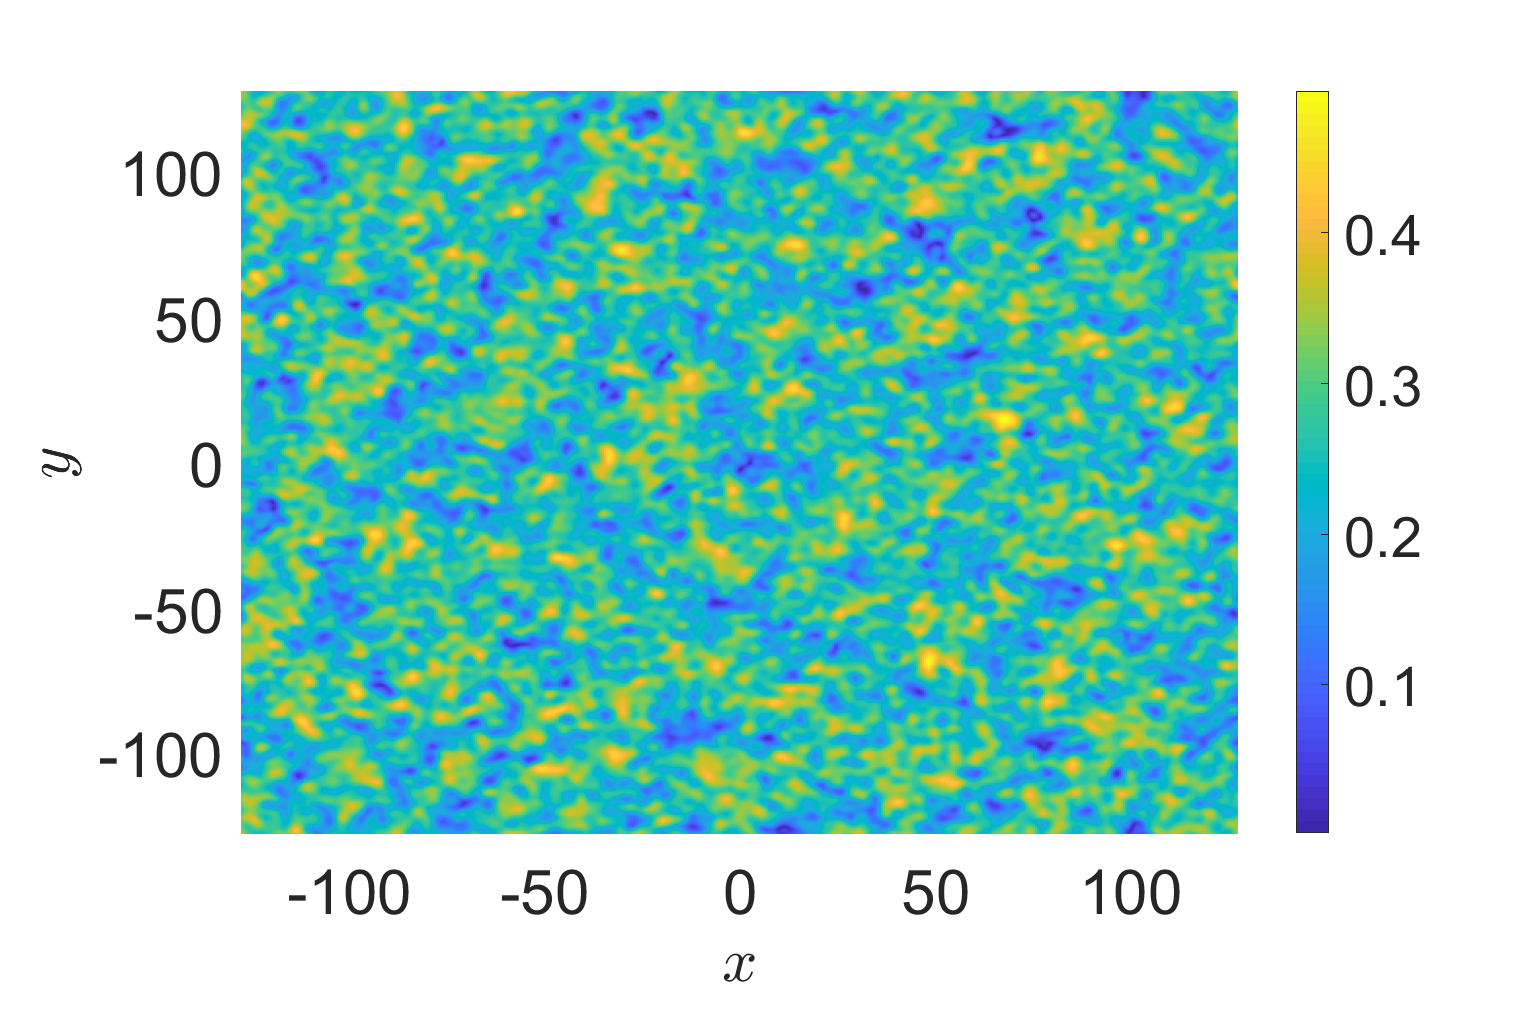
\includegraphics[width=.51\textwidth]{amplitude_wwt_K_256_Lx_128_tf_1pt5e4} &\hspace{-15pt} 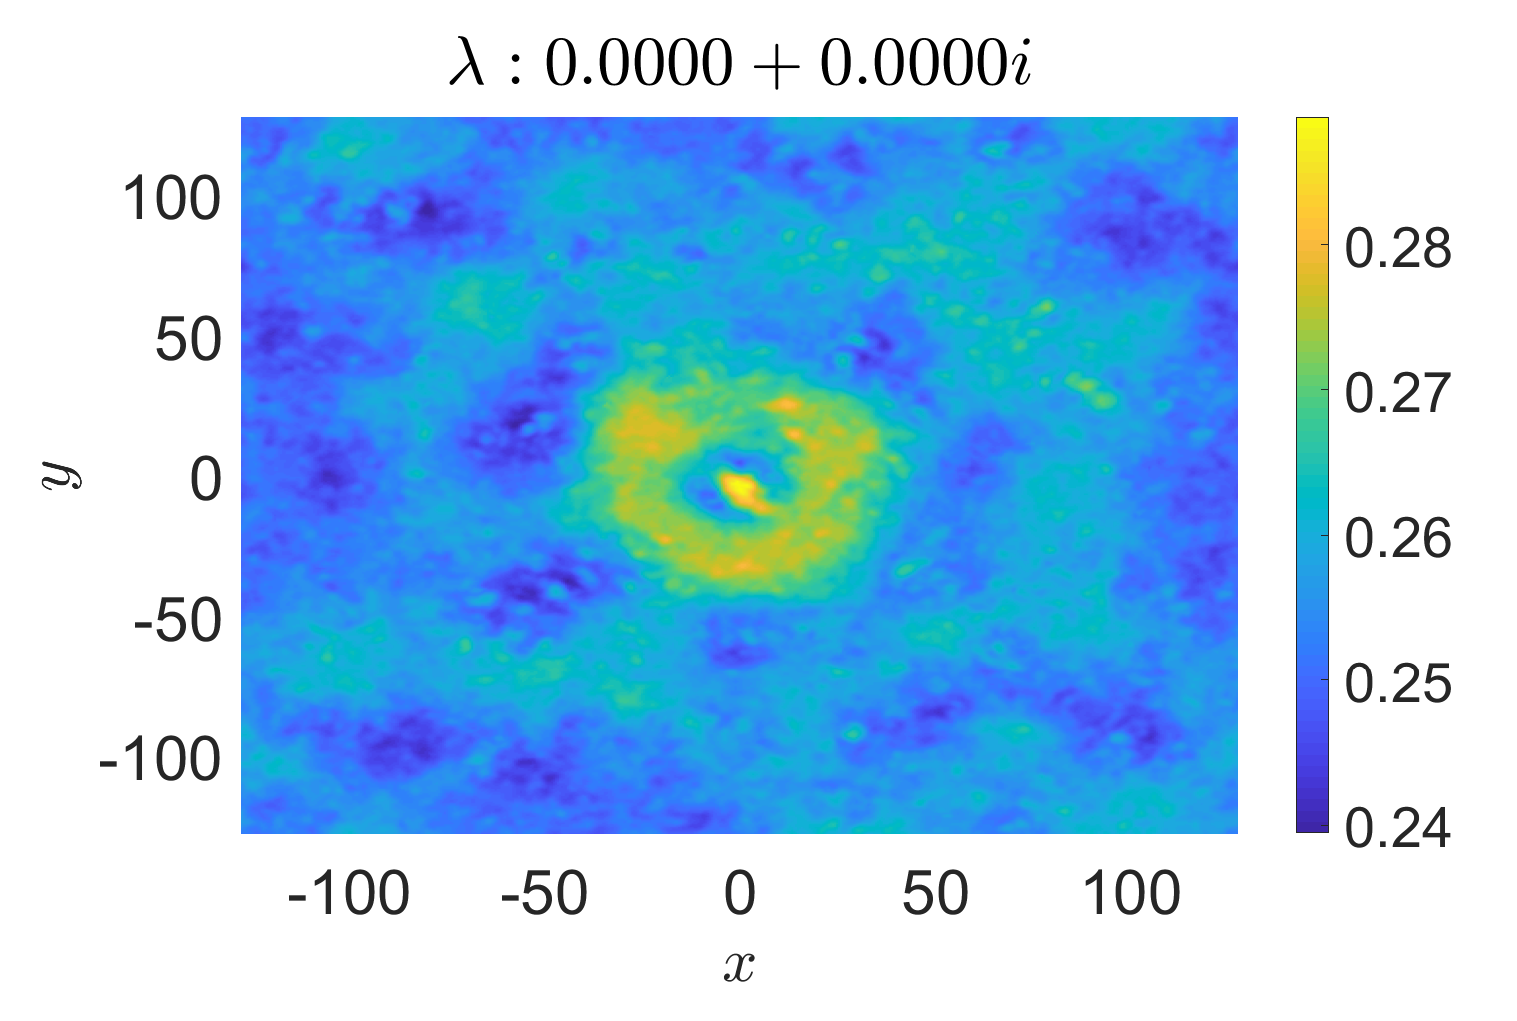
\includegraphics[width=.51\textwidth]{mean_wwt_K_256_Lx_128_tf_1pt5e4} \\
(a) & (b)\\
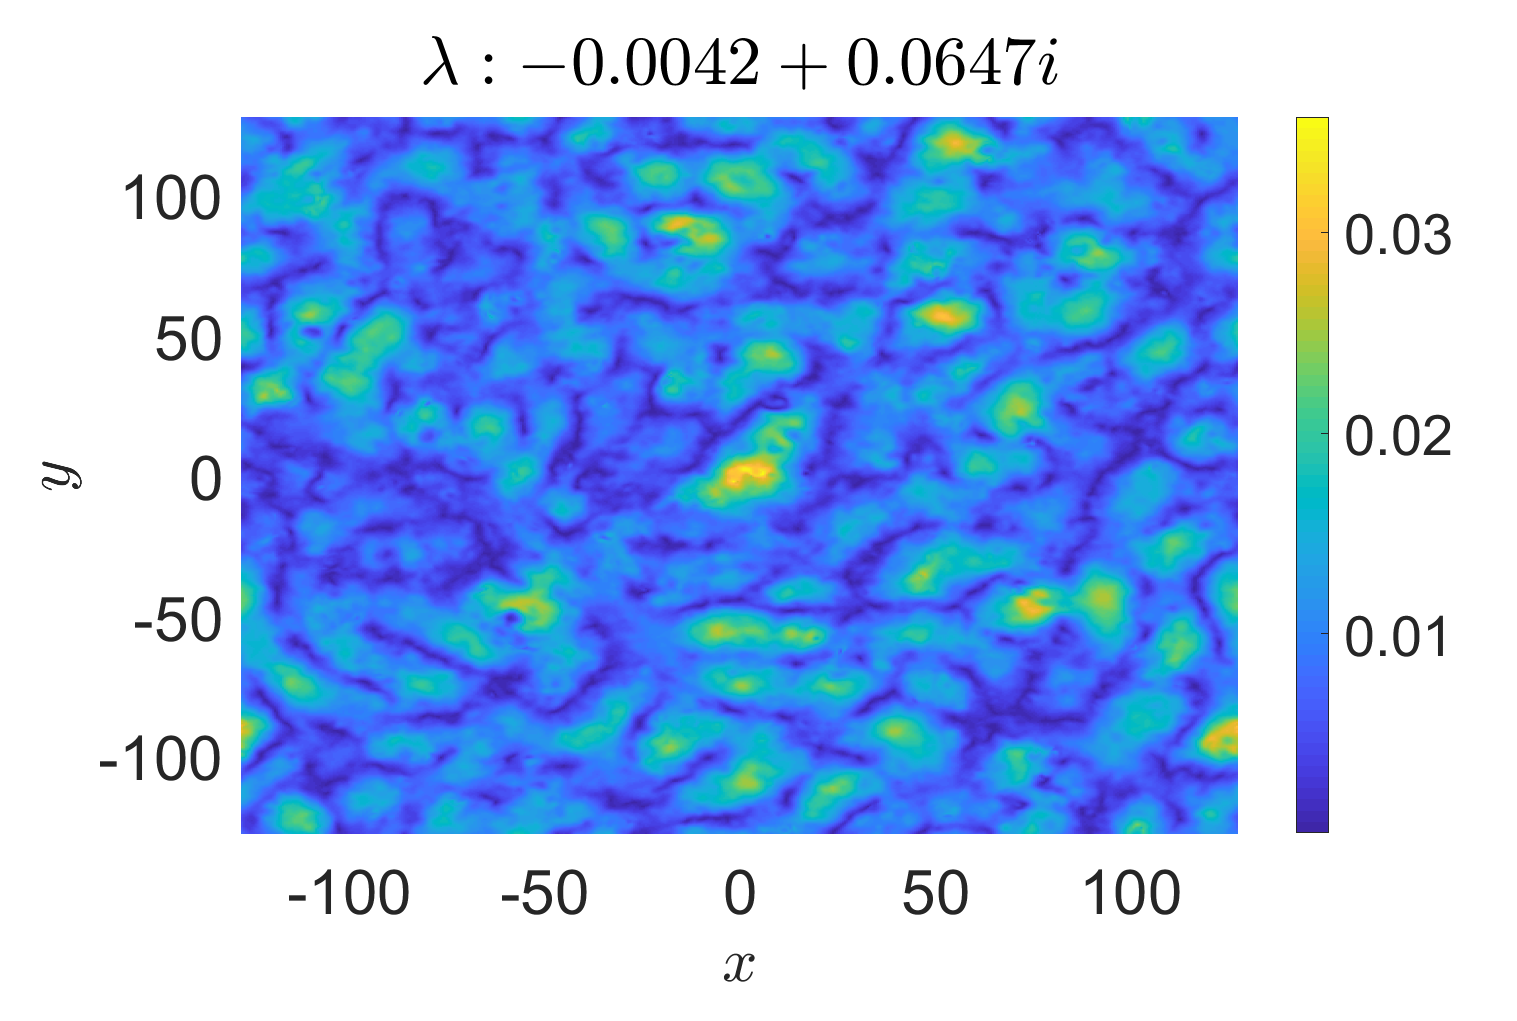
\includegraphics[width=.51\textwidth]{osc1_wwtforce_K_256_Lx_128_tf_1_pt5e4} &\hspace{-15pt} 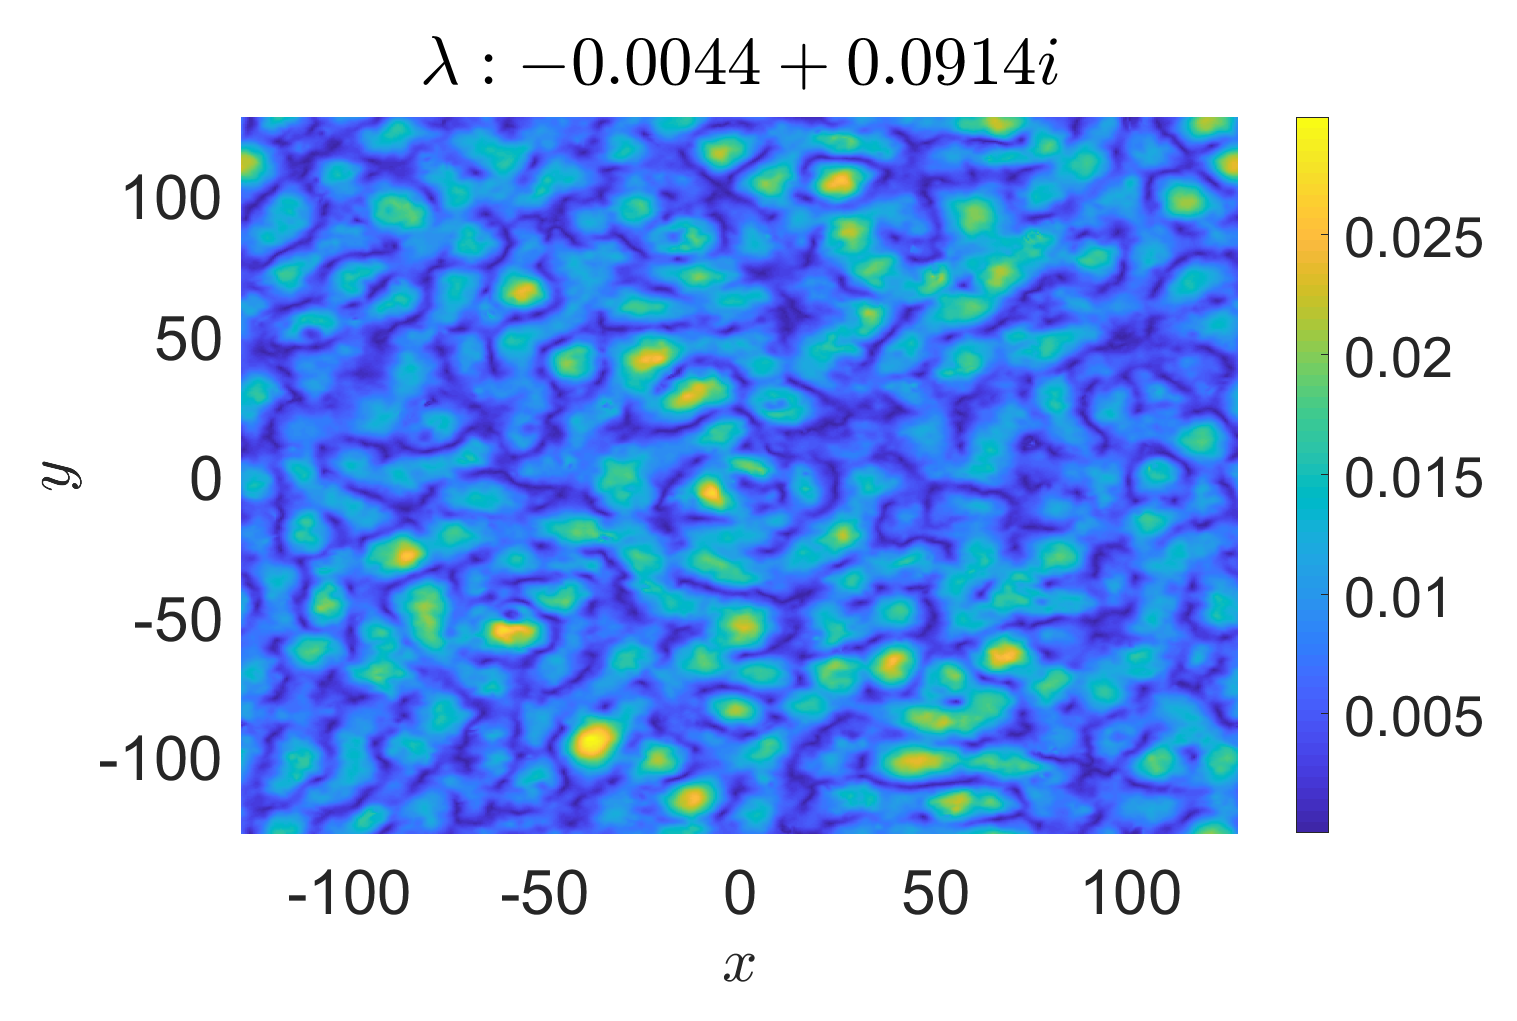
\includegraphics[width=.51\textwidth]{osc2_wwtforce_K_256_Lx_128_tf_1_pt5e4} \\
(c) & (d)\\
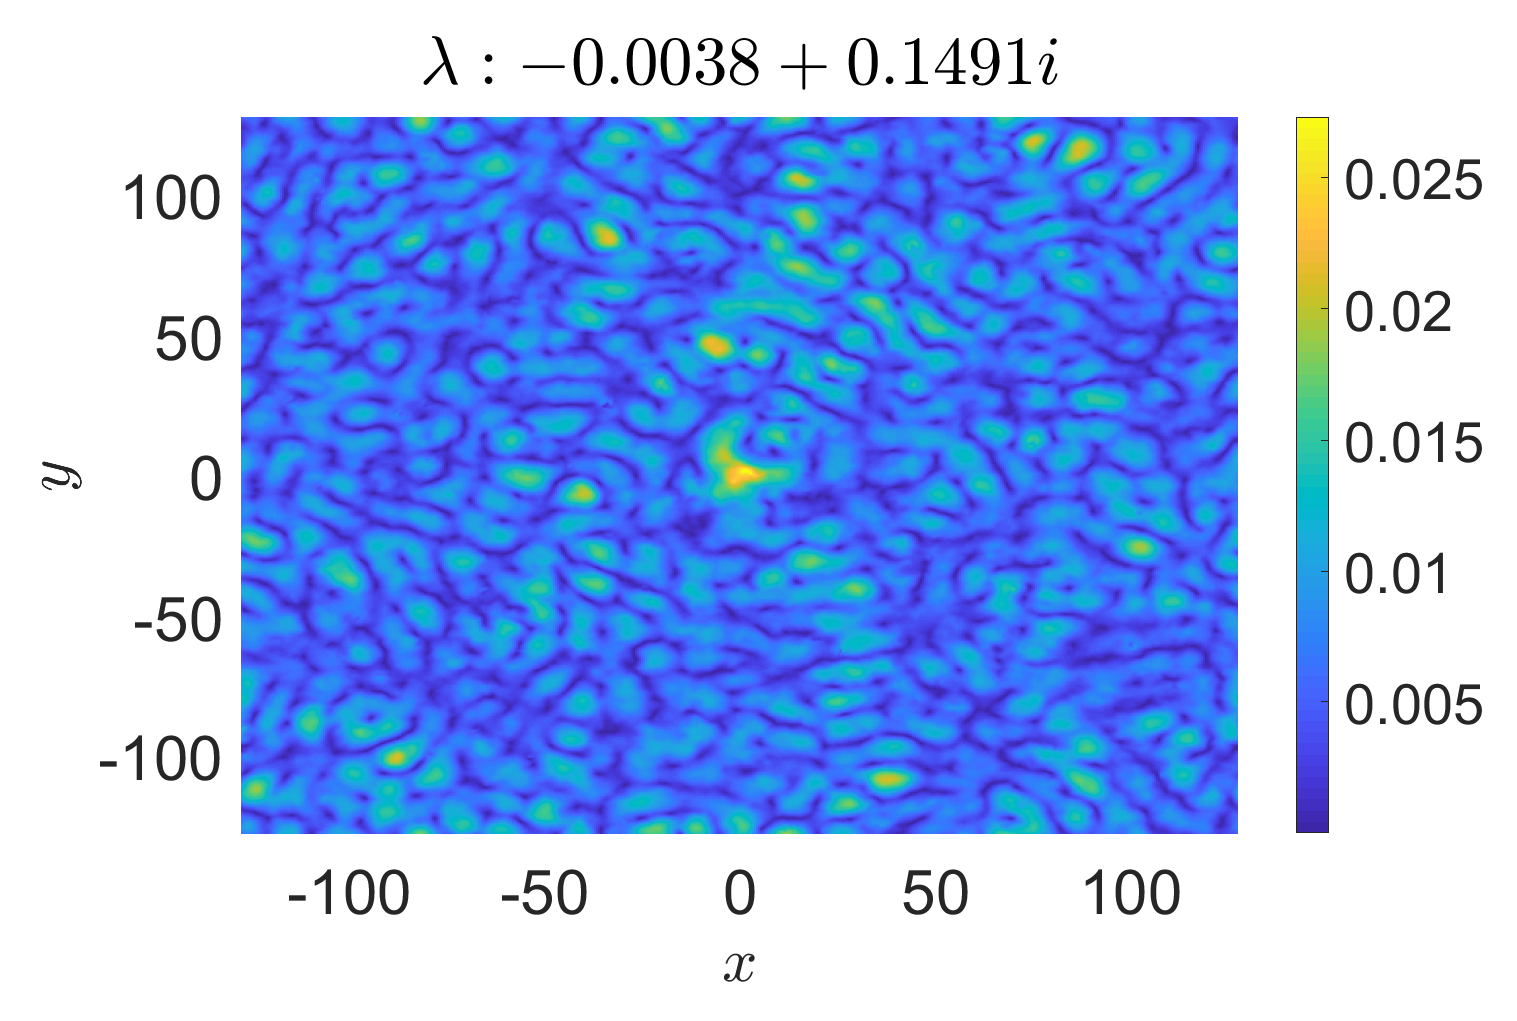
\includegraphics[width=.51\textwidth]{osc3_wwtforce_K_256_Lx_128_tf_1_pt5e4} & \\
(e) & 
\end{tabular}
\caption{The amplitude $\left|\psi(x,y,t_{f})\right|$ (a), weighted mean (b), and next four most signifcant weakly-transient modes (c)-(e) for $k_{l}=4$, $k_{h}=6$, $\gamma_{0}=2.1\times 10^{-3}$. }
\label{fig:ampcompwwt}
\end{figure}

\subsubsection*{Low-Frequency Saturation Case}
Through the remaining simulations, we remove the hypoviscosity, and let $\gamma_{0}=2.1\times 10^{-3}$, thereby allowing for saturation in longer-wavelengths to occur.  If we continue to look at the relatively low frequency forcing explored above, we expect to see long-wavelength coherent structures to form.  It is at this point that we can plainly see the advantage of using the DMD by comparing the fully evolved solution to the NLS equation in Figure \ref{fig:ampcomplf} (a) to the mean DMD mode in Figure \ref{fig:ampcomplf} (b).  The mean mode clearly identifies a finite number of vortices interacting through a finite amplitude background.  
\begin{figure}[!ht]
\centering
\begin{tabular}{cc}
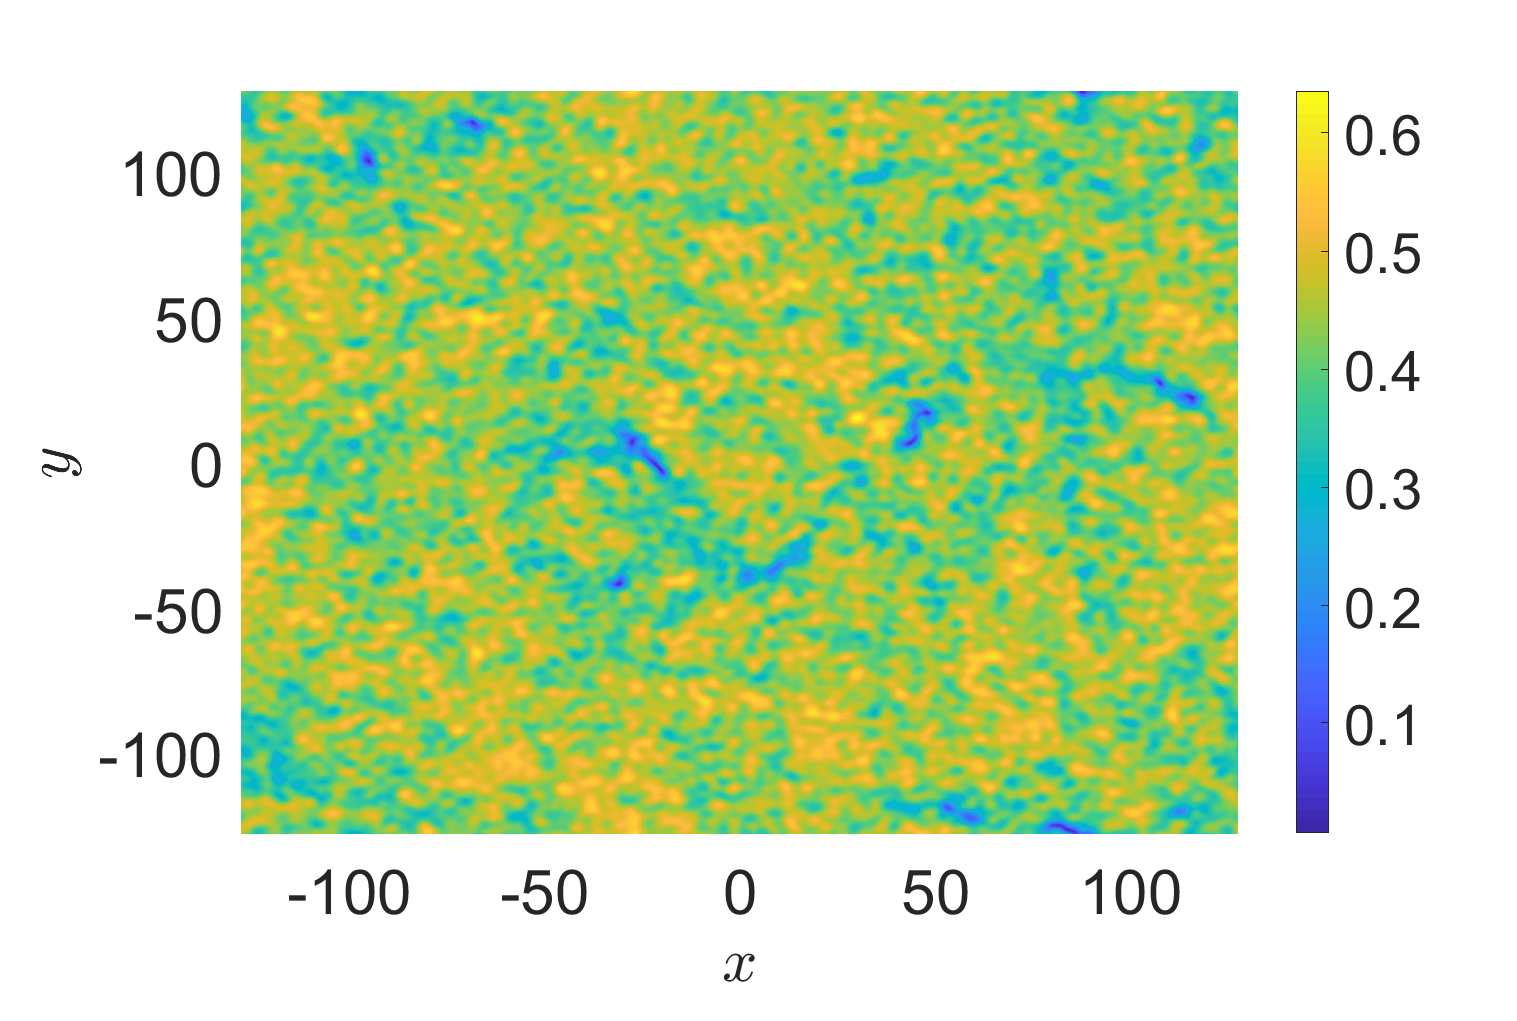
\includegraphics[width=.51\textwidth]{amplitude_lfforce_K_256_Lx_128_tf_1pt5e4} &\hspace{-15pt} 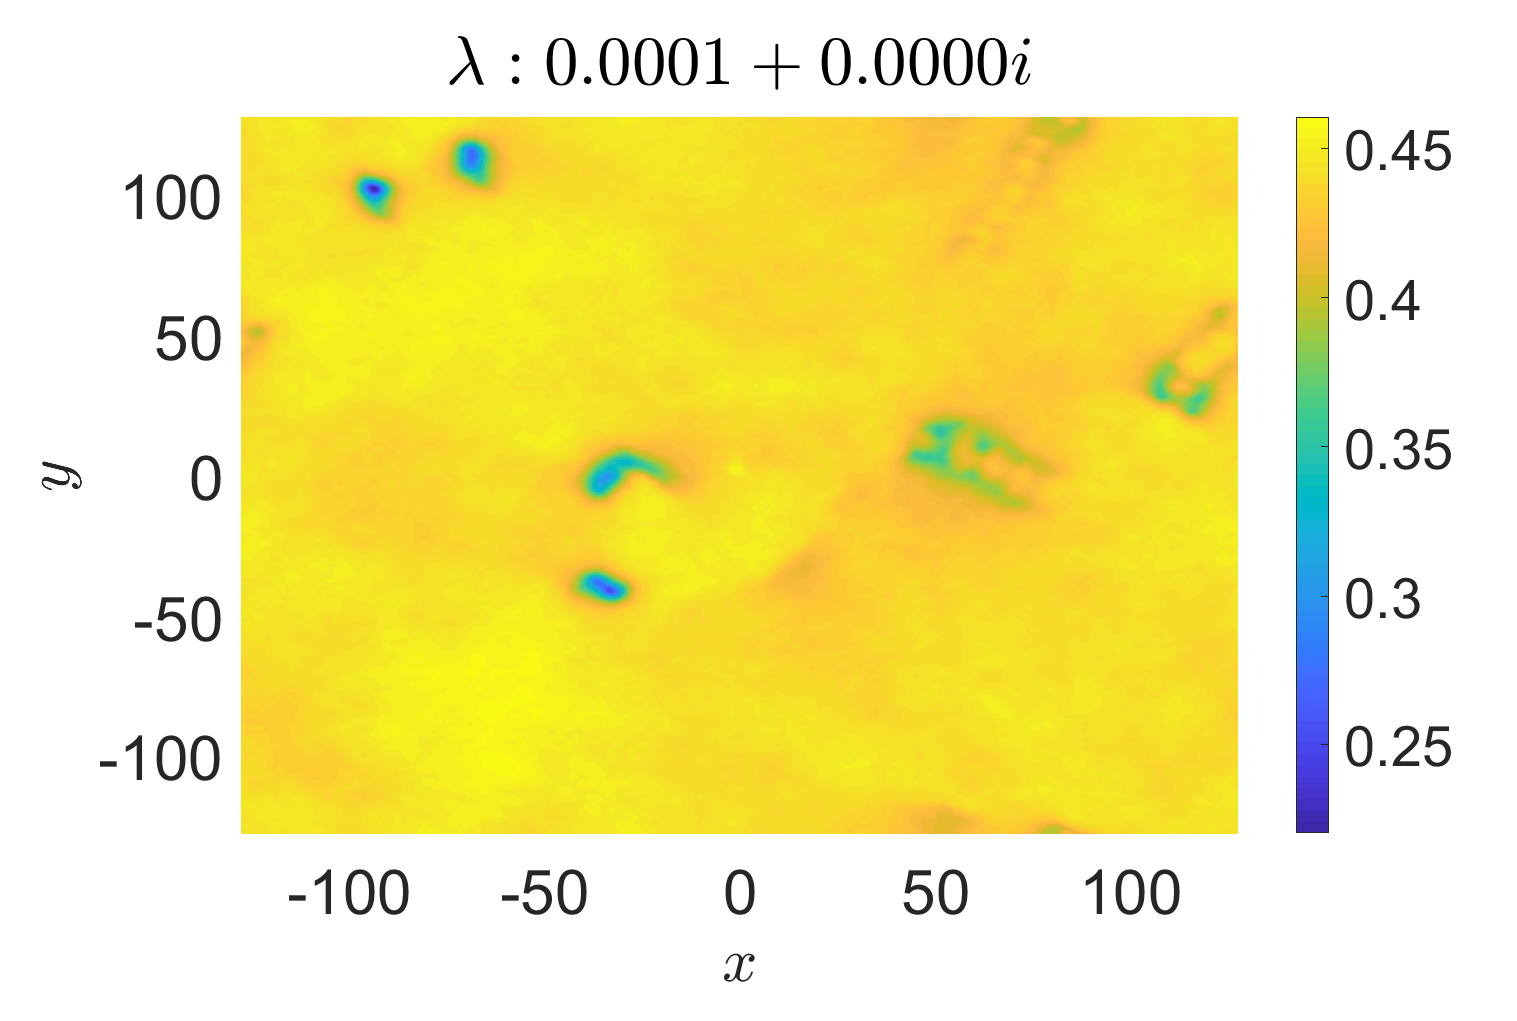
\includegraphics[width=.51\textwidth]{mean_lfforce_K_256_Lx_128_tf_1_pt5e4} \\
(a) & (b)\\
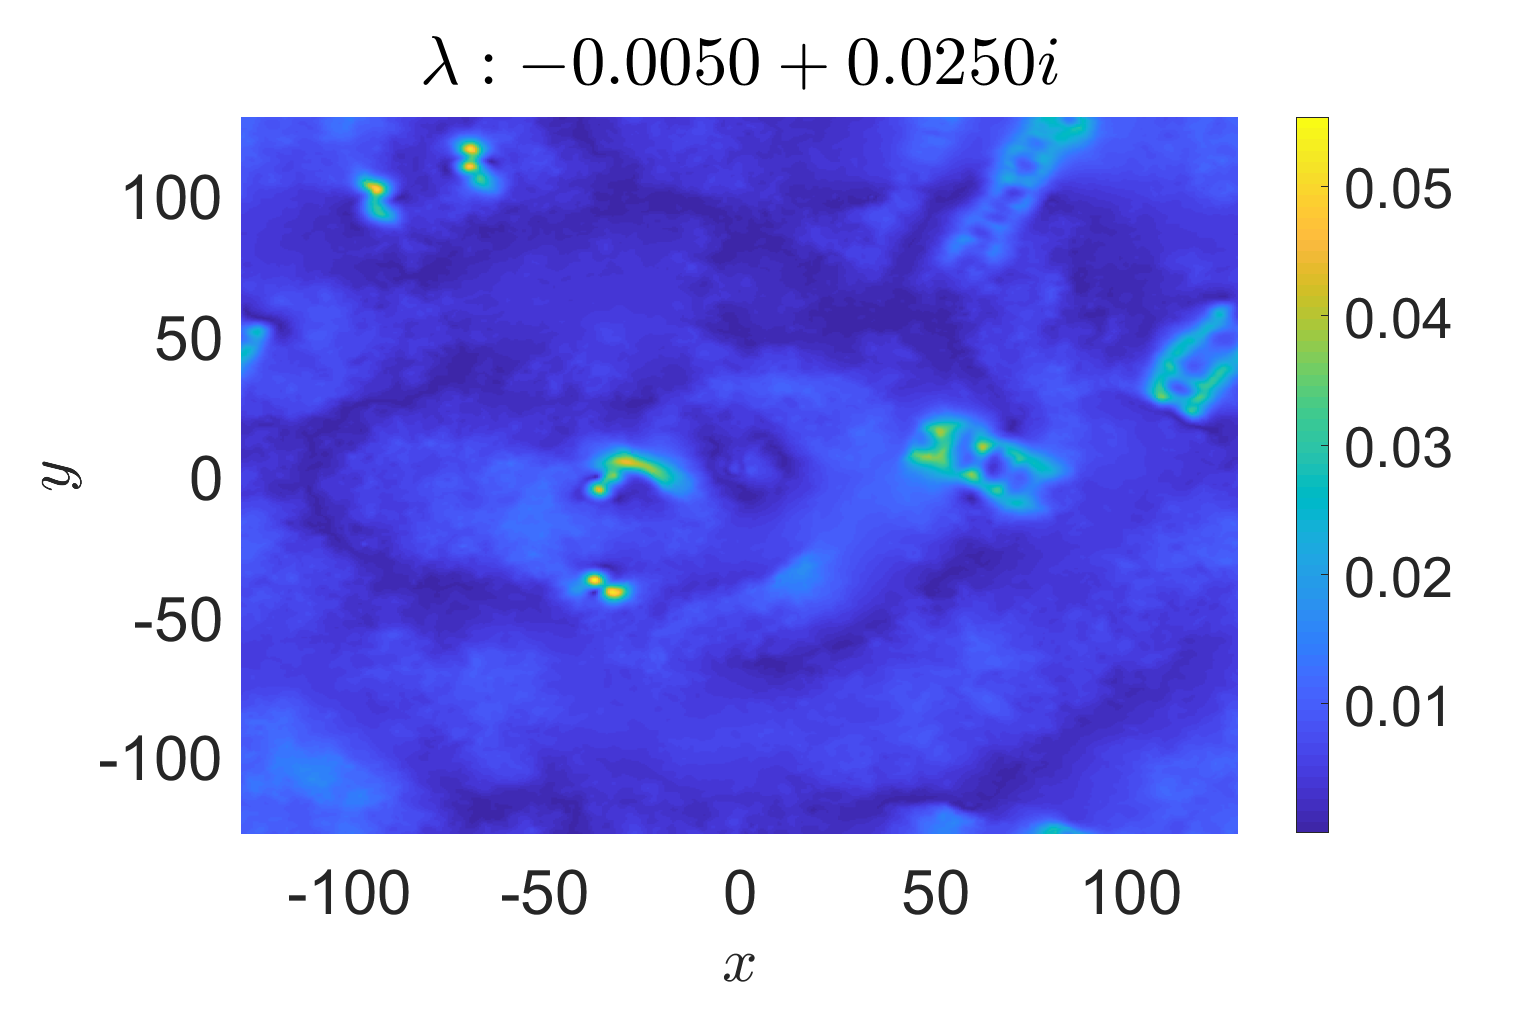
\includegraphics[width=.51\textwidth]{osc1_lfforce_K_256_Lx_128_tf_1_pt5e4} &\hspace{-15pt} 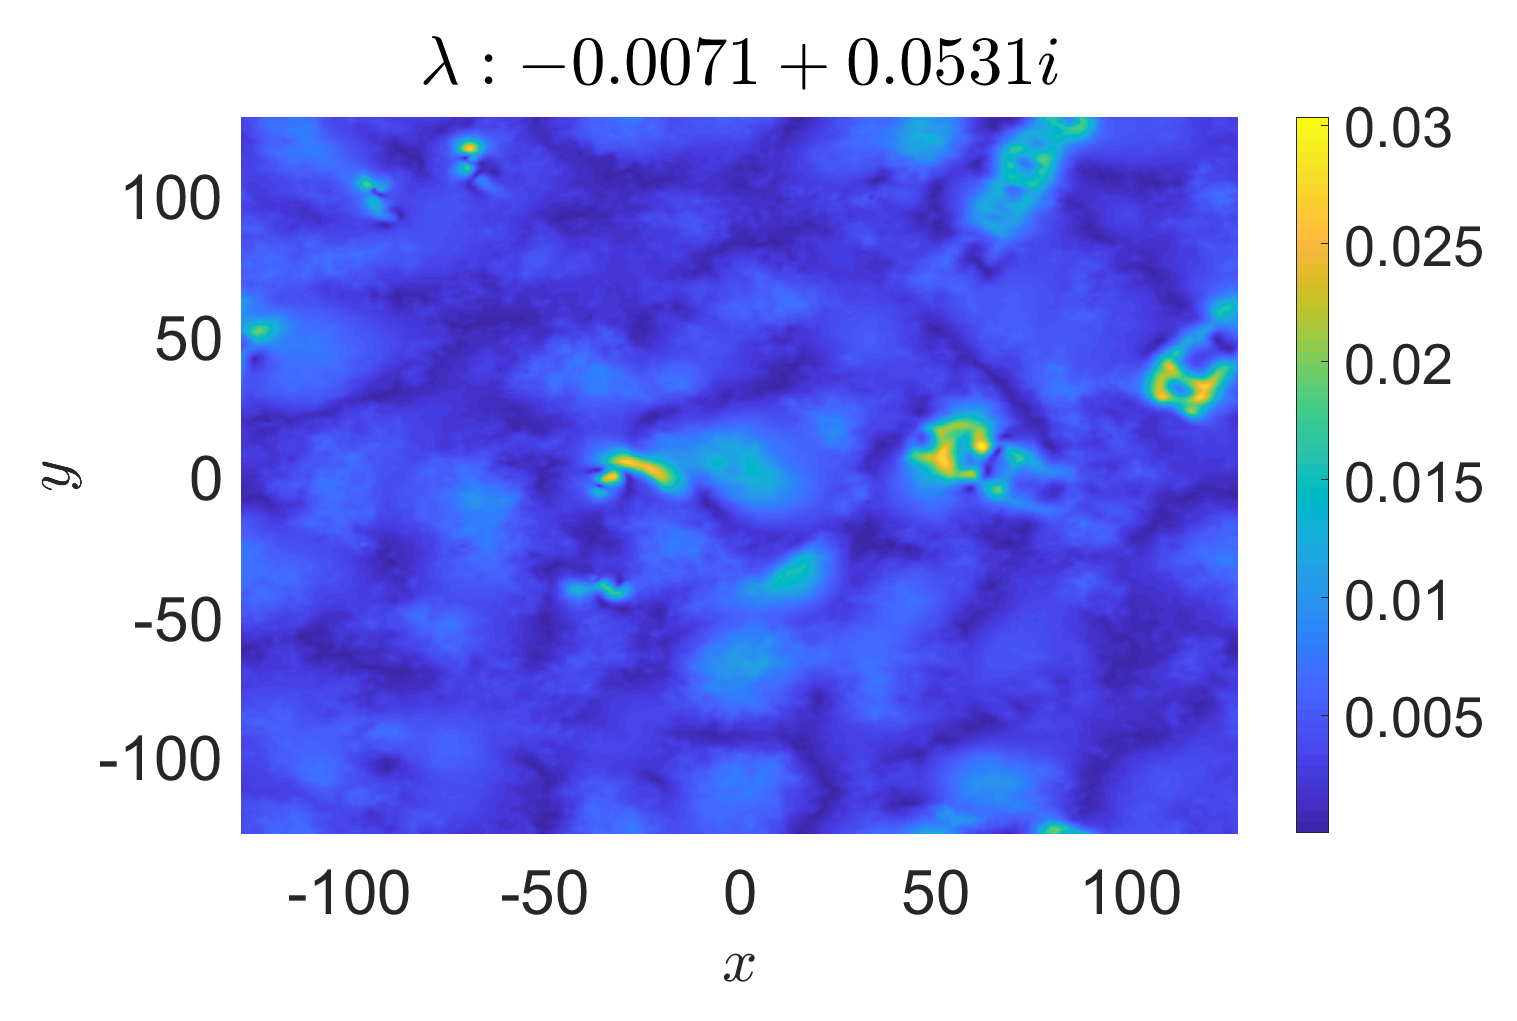
\includegraphics[width=.51\textwidth]{osc2_lfforce_K_256_Lx_128_tf_1_pt5e4} \\
(c) & (d)\\
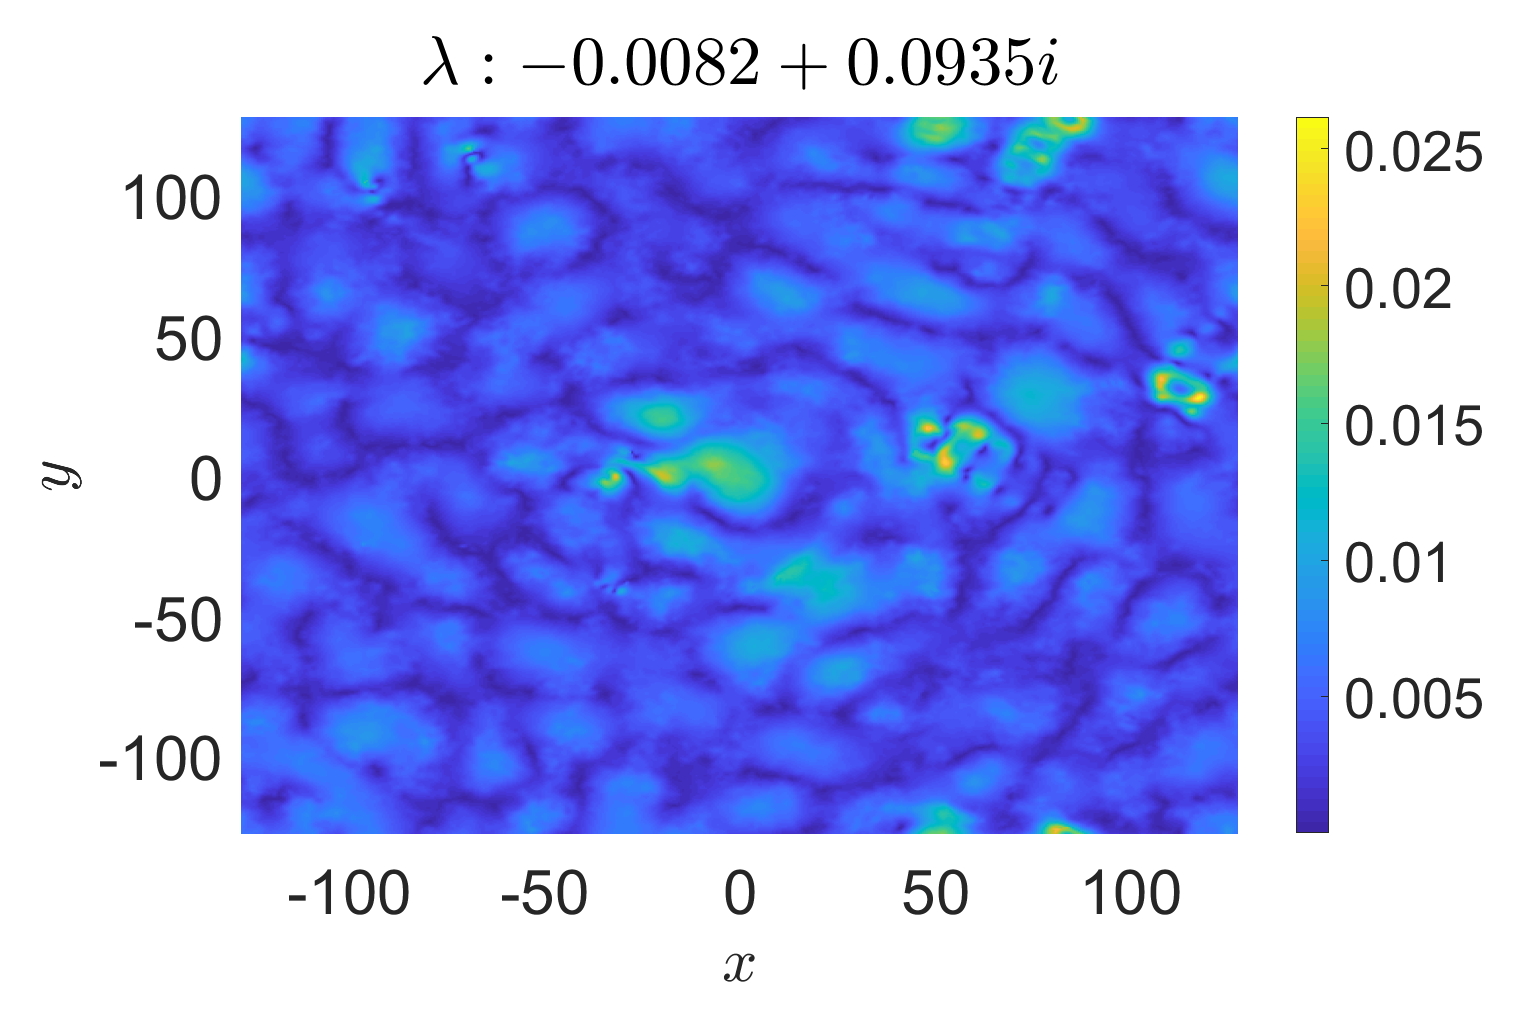
\includegraphics[width=.51\textwidth]{osc3_lfforce_K_256_Lx_128_tf_1_pt5e4} & \\
(e) & 
\end{tabular}
\caption{The amplitude $\left|\psi(x,y,t_{f})\right|$ (a), weighted mean (b), and next four most signifcant weakly-transient modes (c)-(e) for $k_{l}=4$, $k_{h}=6$, $\gamma_{0}=2.1\times 10^{-3}$. }
\label{fig:ampcomplf}
\end{figure}

Of interest though is the relative similarity in the finer, higher-frequency features seen in Figures \ref{fig:ampcomplf} (c)-(f) to those in Figures \ref{fig:ampcompwwt} (c)-(f).  As seen, they are relatively siimilar in terms of their overall characteristics, and thus we can characterize the low-frequency saturation case as a long-wave condensed mean with a weakly-turbulent background fluctuating about this mean.  

\subsubsection*{High-Frequency Saturation Case}
We now look at higher-frequency forcing where we let $k_{l}=60$ and $k_{h}=63$.  As in the low-frequency, long-wavelength saturated case above, we see that the mean DMD mode seen in Figure \ref{fig:ampcomphf} (b) clearly isolates the condensed dynamics obscured through the higher-frequency spatial features in the solution to the NLS equation seen in Figure \ref{fig:ampcomphf} (a).  In contrast the low-frequency forcing case above though, we see in the higher-order modes in Figures \ref{fig:ampcomphf} (c)-(f), far sharper, or higher-frequency, spatial features, thus clearly reflecting the different forcing mechanism in play in this simulation.   
\begin{figure}[!ht]
\centering
\begin{tabular}{cc}
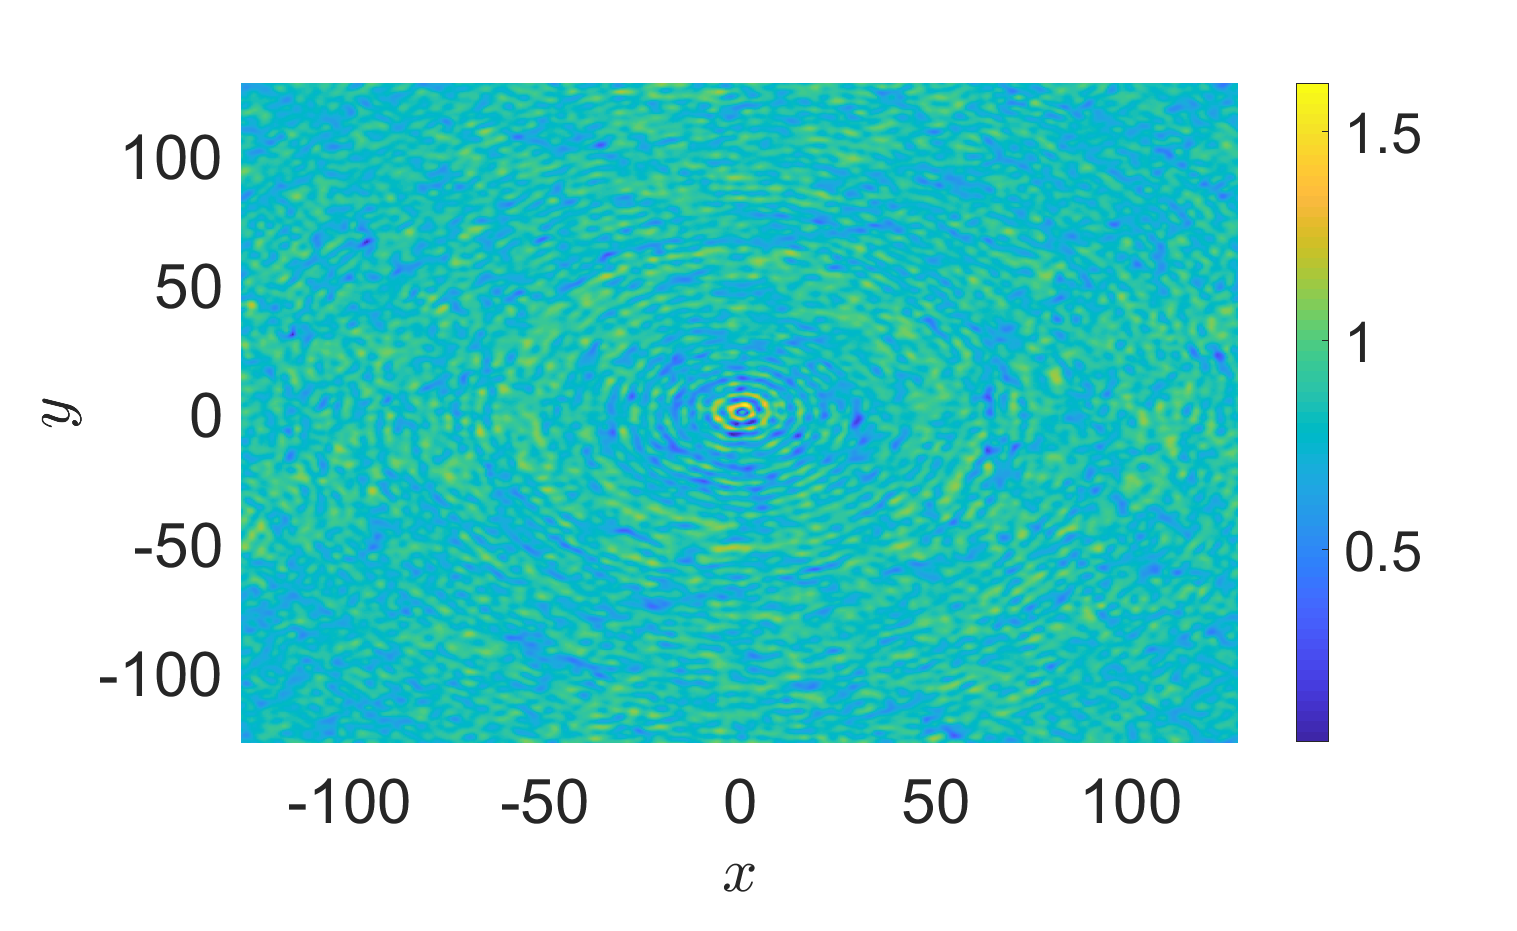
\includegraphics[width=.525\textwidth]{amplitude_hfforce_K_256_Lx_128_tf_2e4} &\hspace{-15pt} 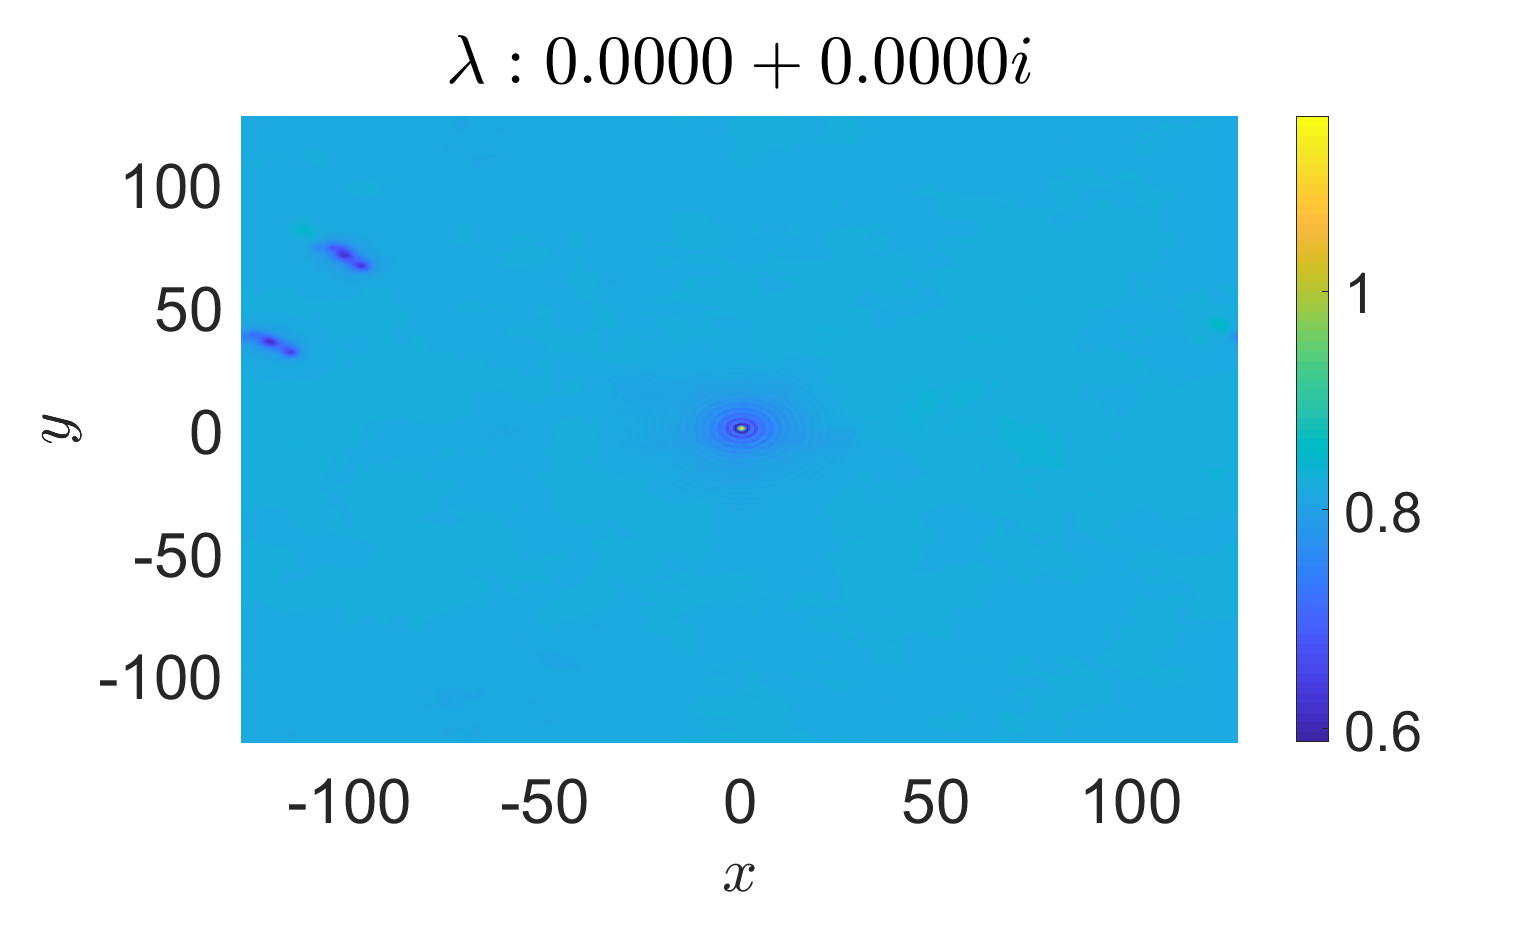
\includegraphics[width=.51\textwidth]{mean_hfforce_K_256_Lx_128_tf_2e4} \\
(a) & (b)\\
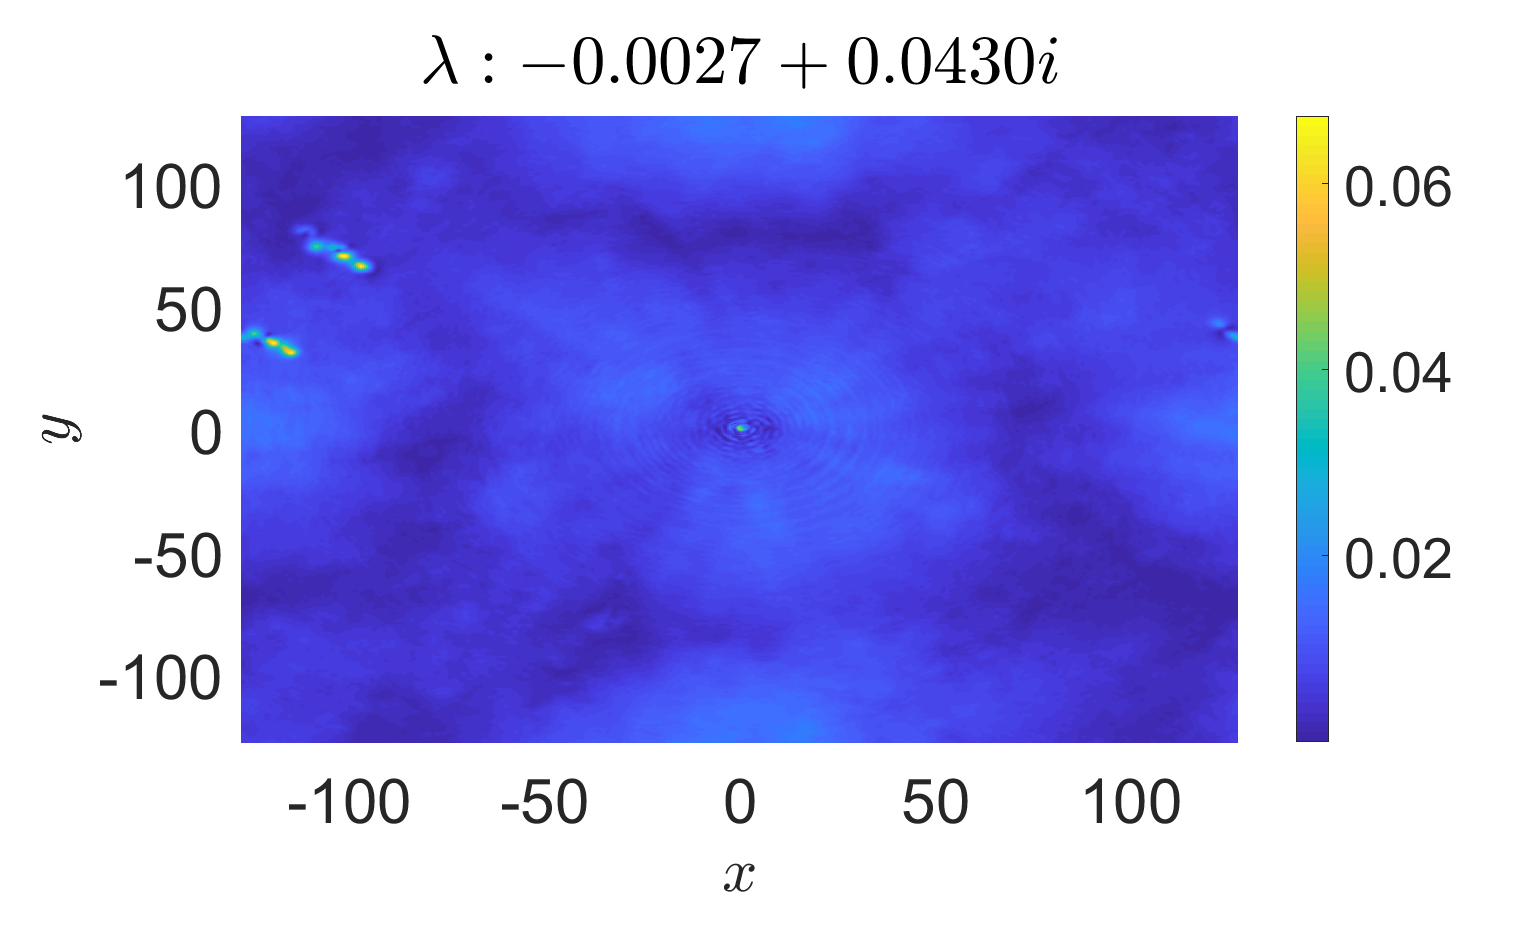
\includegraphics[width=.525\textwidth]{osc1_hfforce_K_256_Lx_128_tf_2e4} &\hspace{-15pt} 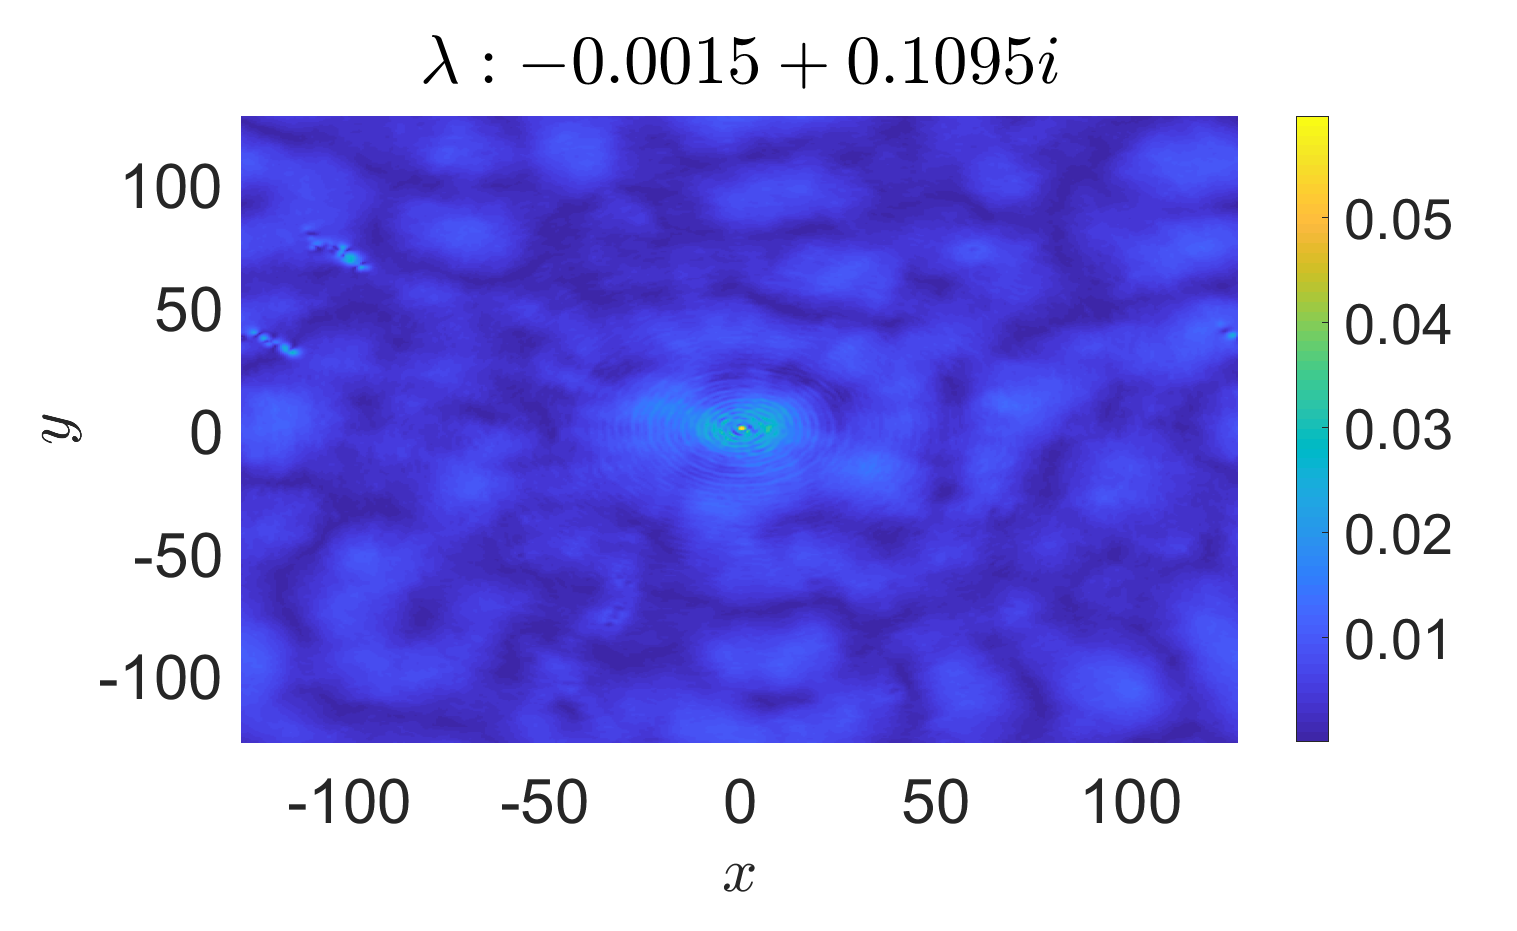
\includegraphics[width=.51\textwidth]{osc2_hfforce_K_256_Lx_128_tf_2e4} \\
(c) & (d)\\
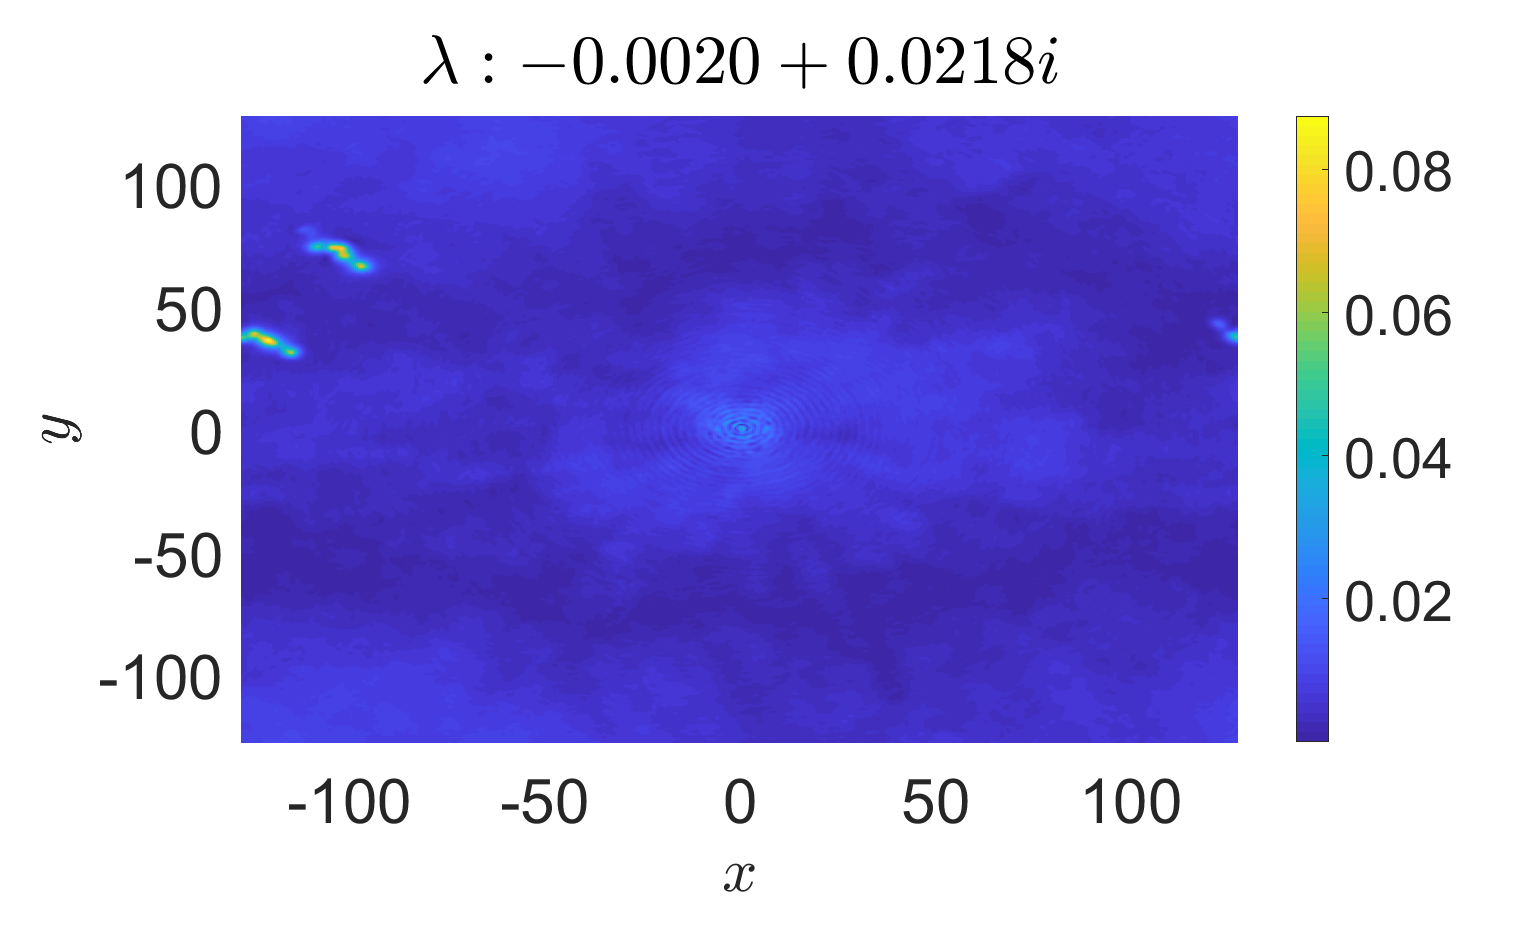
\includegraphics[width=.525\textwidth]{osc3_hfforce_K_256_Lx_128_tf_2e4} & \\
(e) & 
\end{tabular}
\caption{The amplitude $\left|\psi(x,y,t_{f})\right|$ (a), weighted mean (b), and next four most signifcant weakly-transient modes (c)-(f) for $k_{l}=60$, $k_{h}=63$, $\gamma_{0}=2.1\times 10^{-3}$. }
\label{fig:ampcomphf}
\end{figure}

\subsection*{Comparison Across Flows via Spectral Characteristics}
We now compare the spectral characteristics and compression ratios of the weak-wave turbulence (WWT), low-frequency saturation (LFS), and high-frequency saturation (HFS) cases studied above.  Here, we focus less on isolating some relatively small number of modes and more examine the charactertistic responses of each measured quantity across the different flows thereby allowing for the identification of classifying features that may not be as readily apparent given the overall complexity of each flow.  
\begin{figure}[!ht]
\centering
\begin{tabular}{cc}
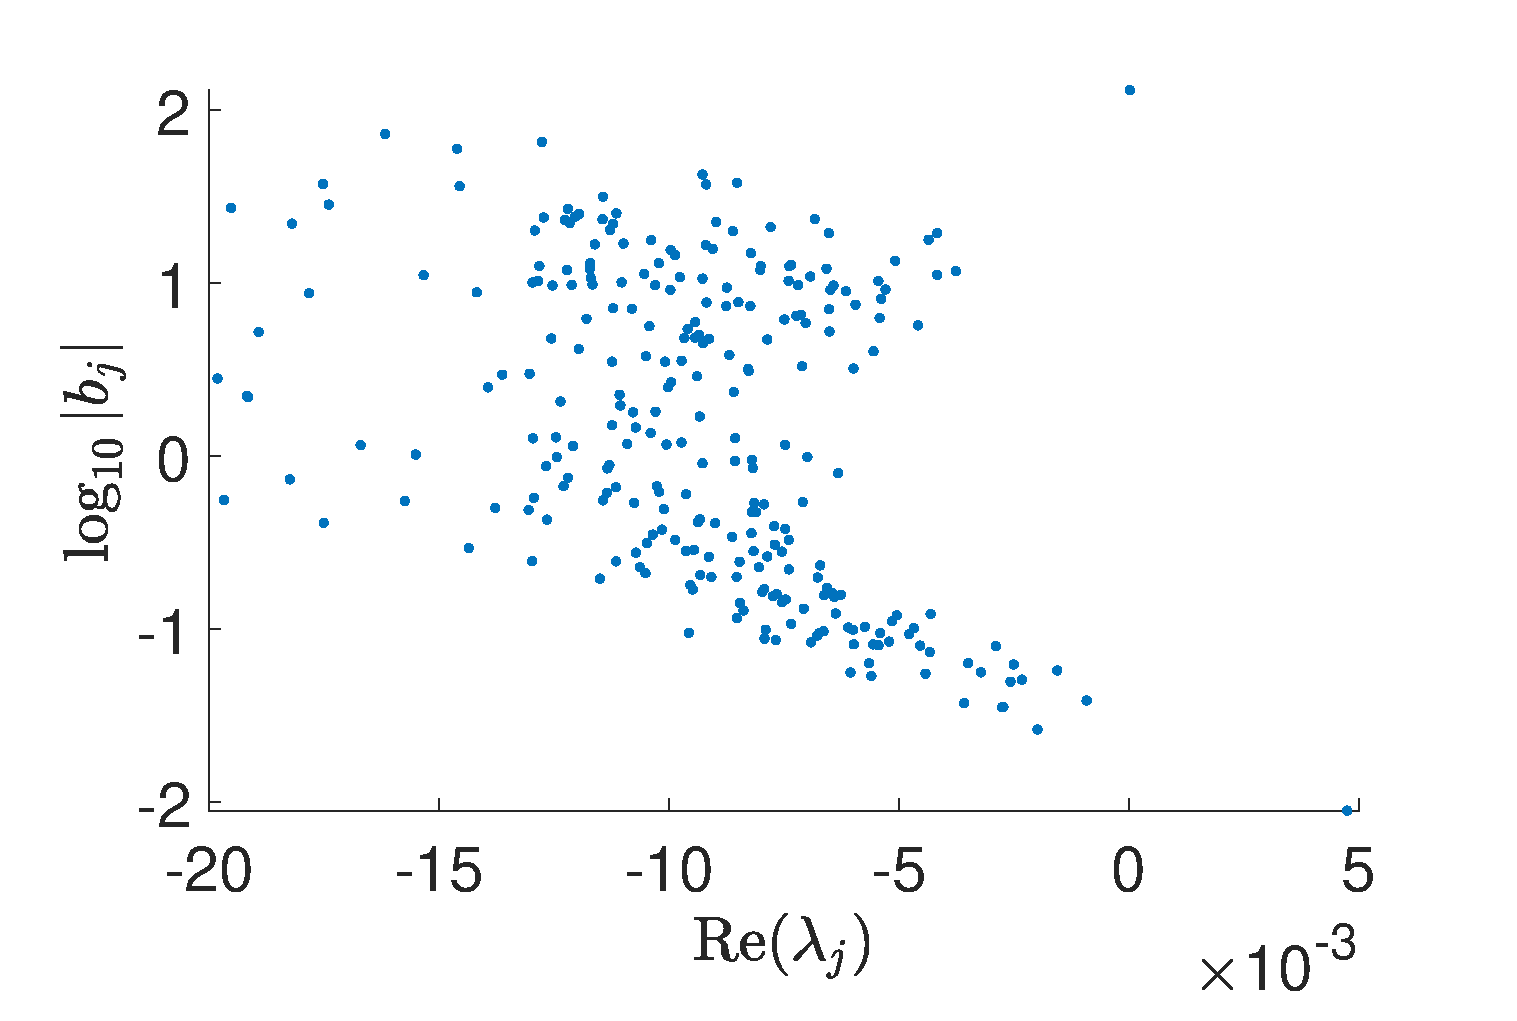
\includegraphics[width=.525\textwidth]{bvals_vs_real_lam_wwtforce_K_256_Lx_128_tf_1_pt5e4} &\hspace{-25pt} 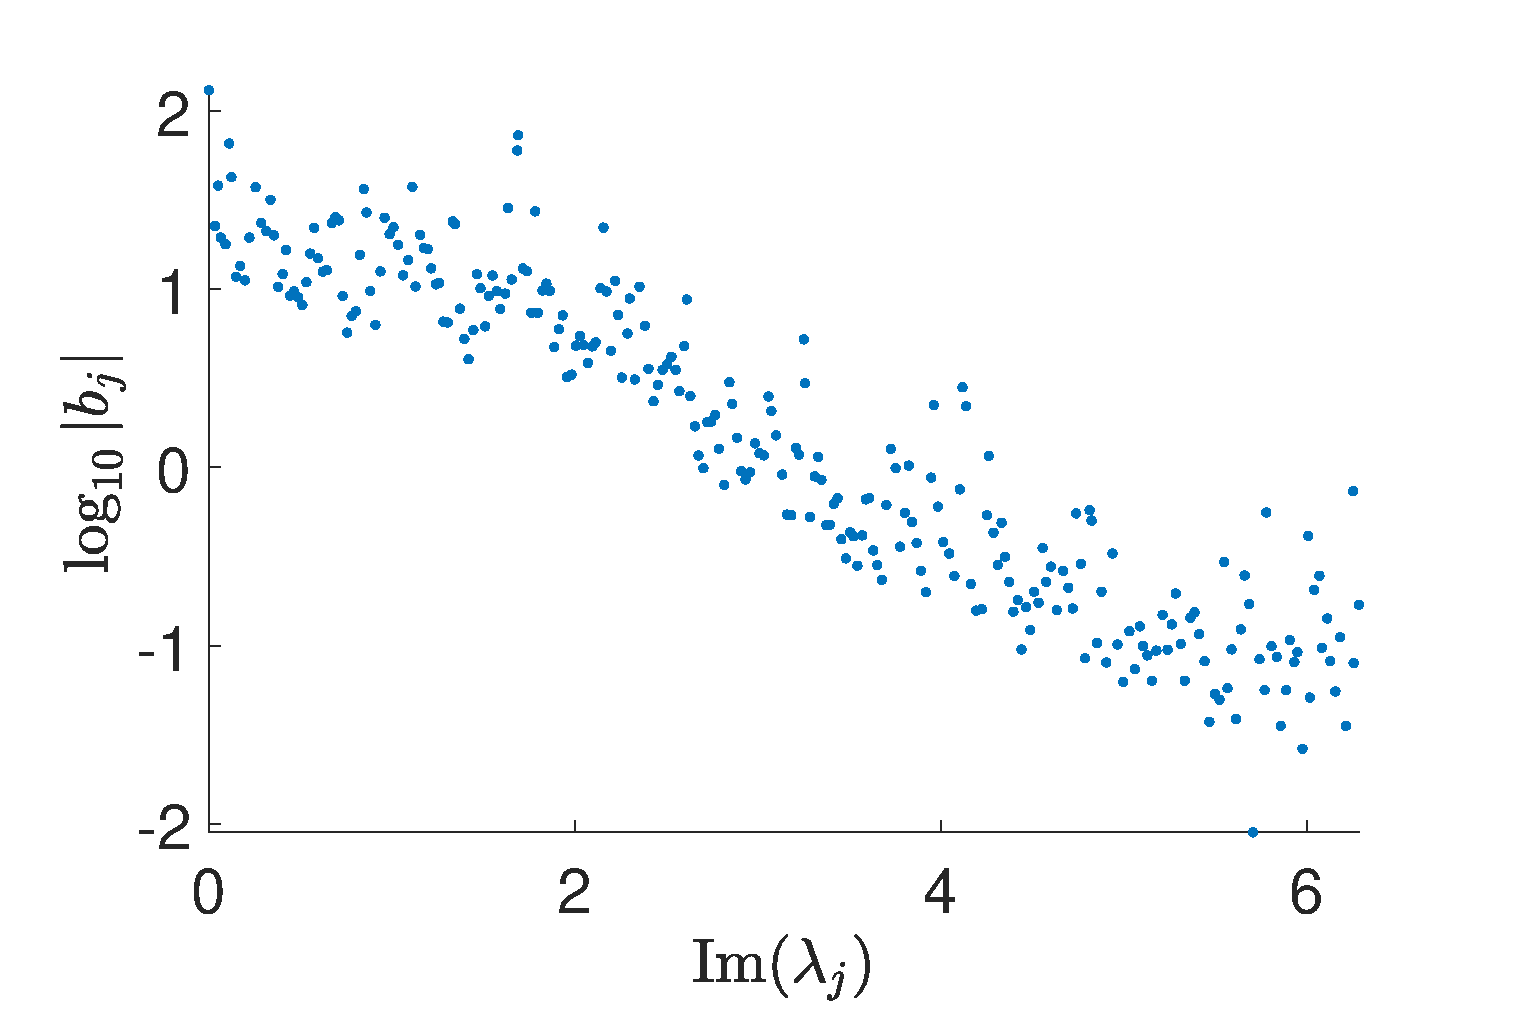
\includegraphics[width=.525\textwidth]{bvals_vs_imag_lam_wwtforce_K_256_Lx_128_tf_1_pt5e4}\\
(a) WWT & (b) WWT\\
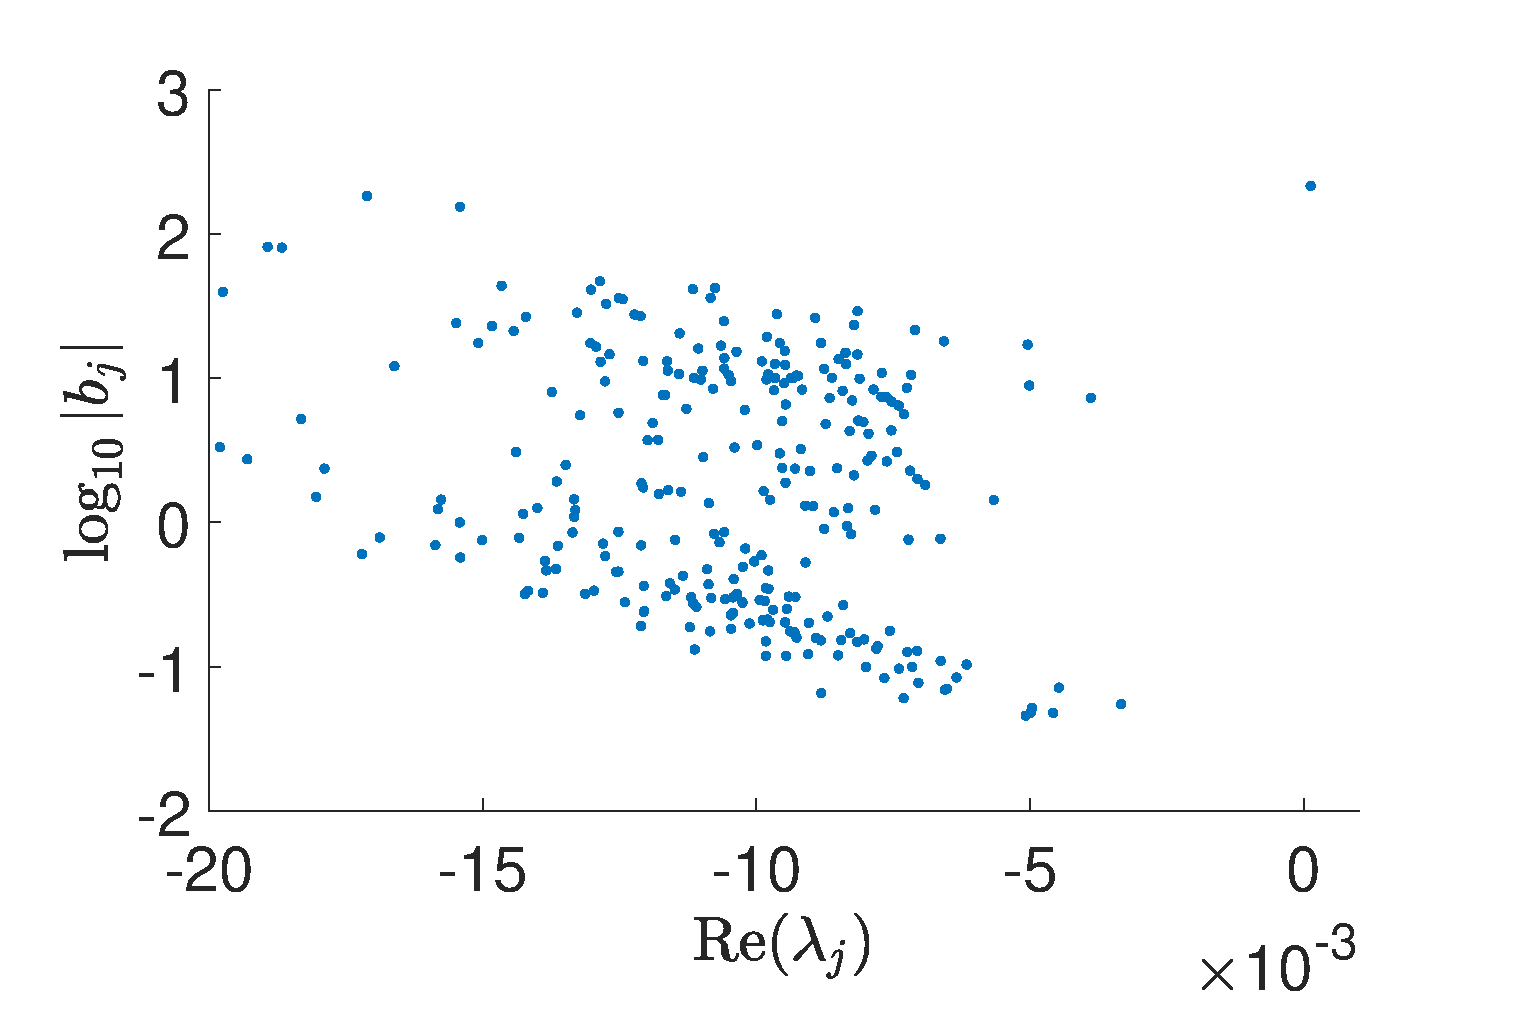
\includegraphics[width=.525\textwidth]{bvals_vs_real_lam_lfforce_K_256_Lx_128_tf_1_pt5e4} &\hspace{-25pt} 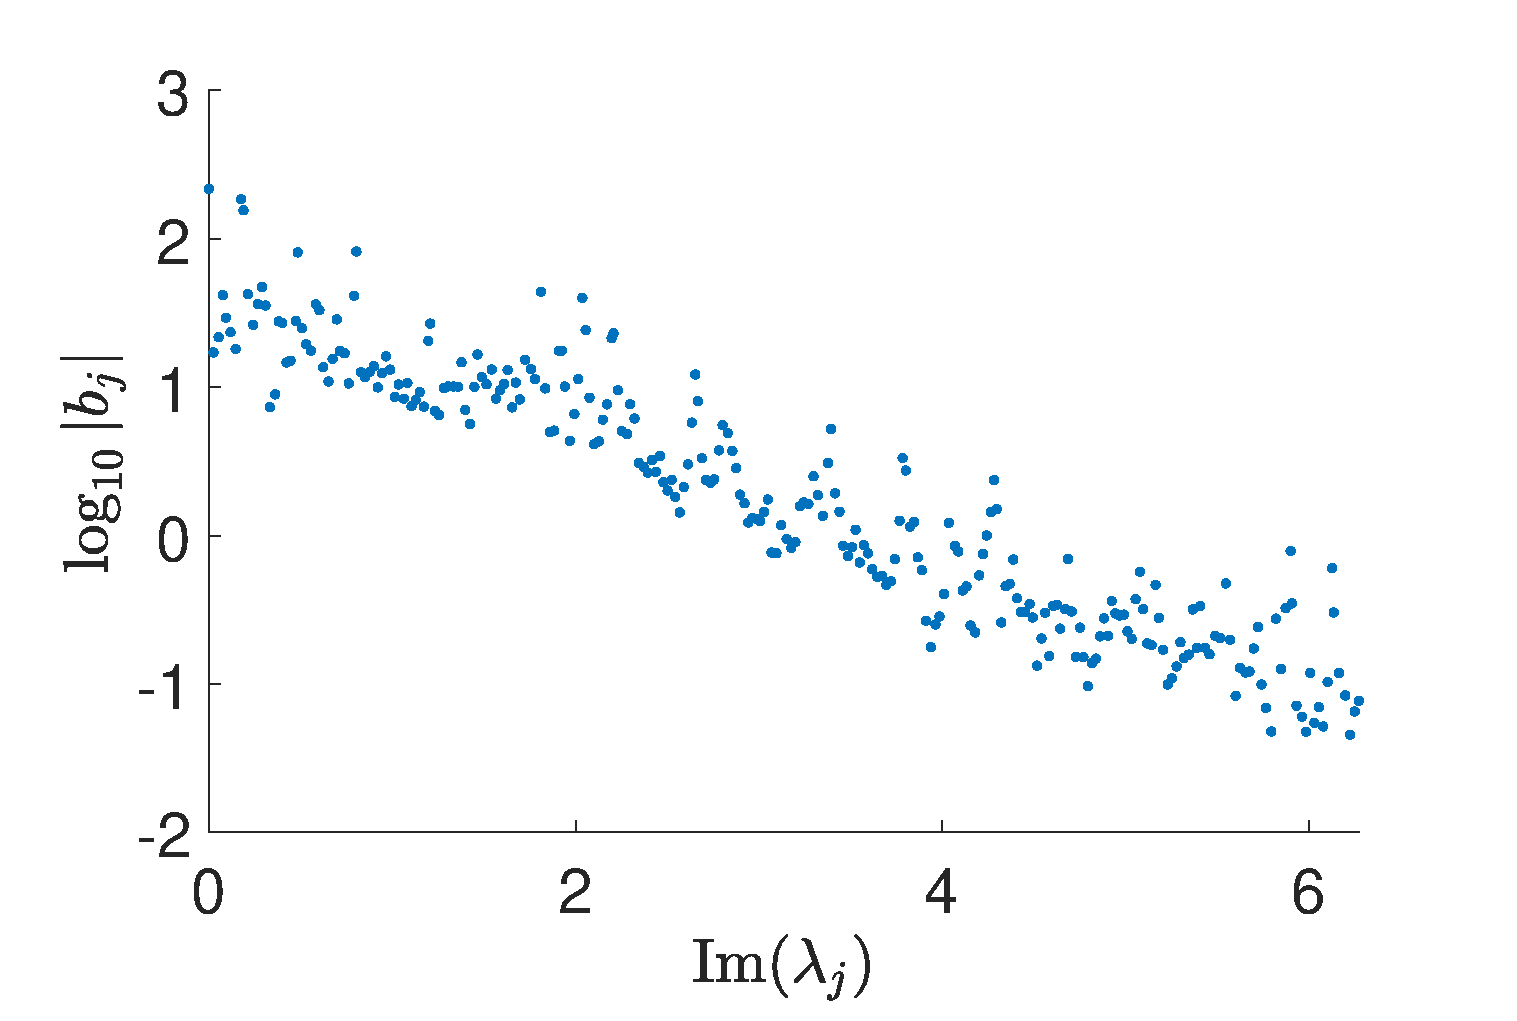
\includegraphics[width=.525\textwidth]{bvals_vs_imag_lam_lfforce_K_256_Lx_128_tf_1_pt5e4}\\
(c) LFS & (d) LFS\\
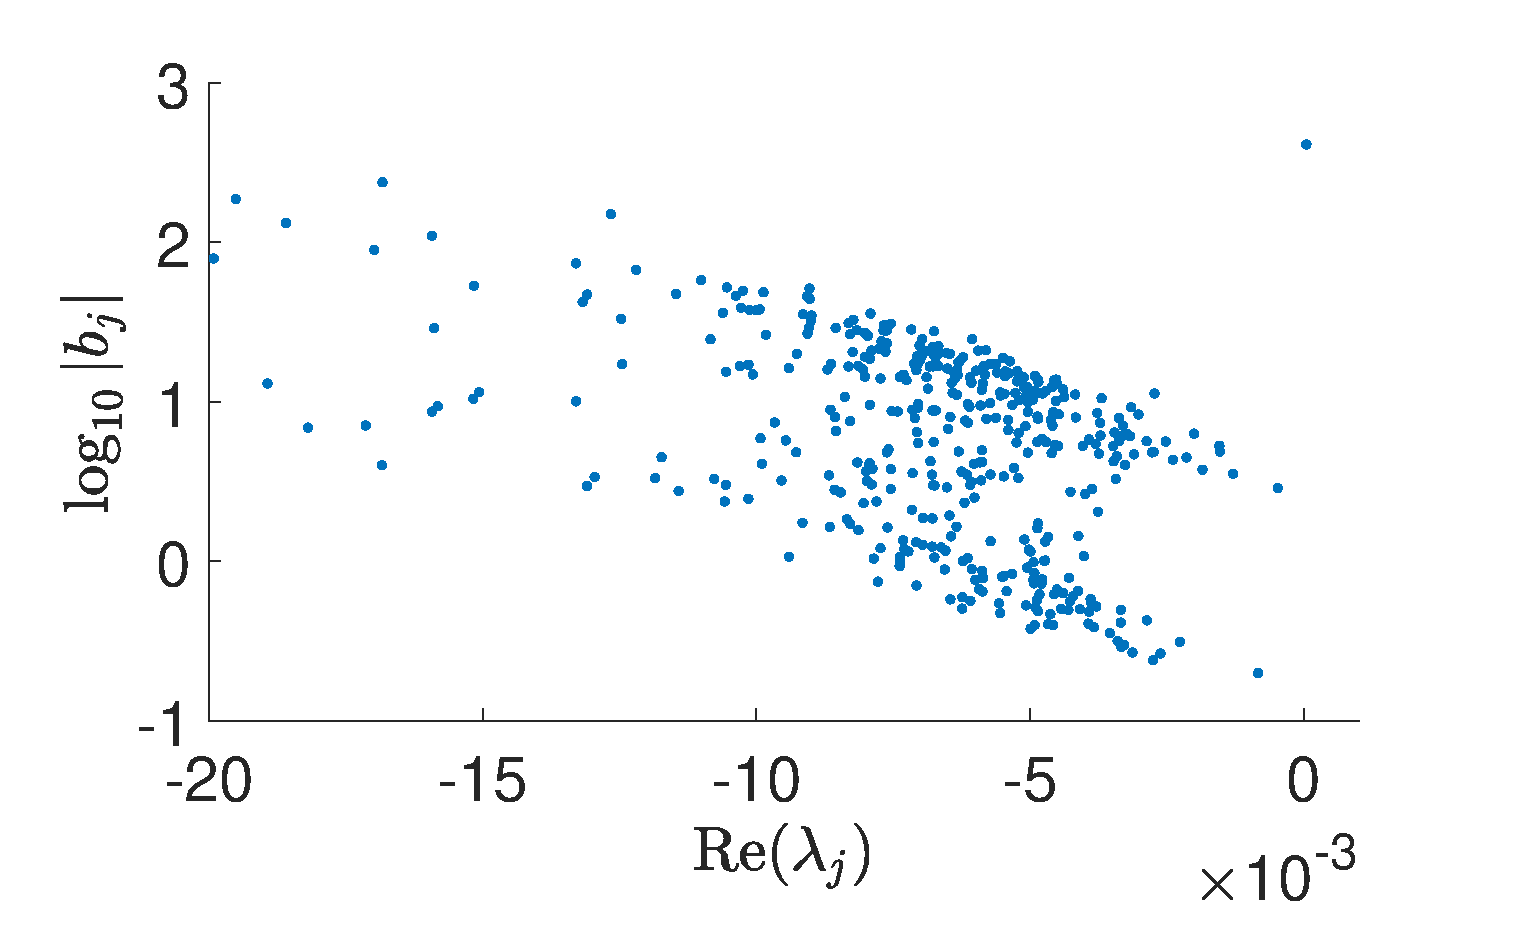
\includegraphics[width=.525\textwidth]{bvals_vs_real_lam_hfforce_K_256_Lx_128_tf_2e4} &\hspace{-25pt} 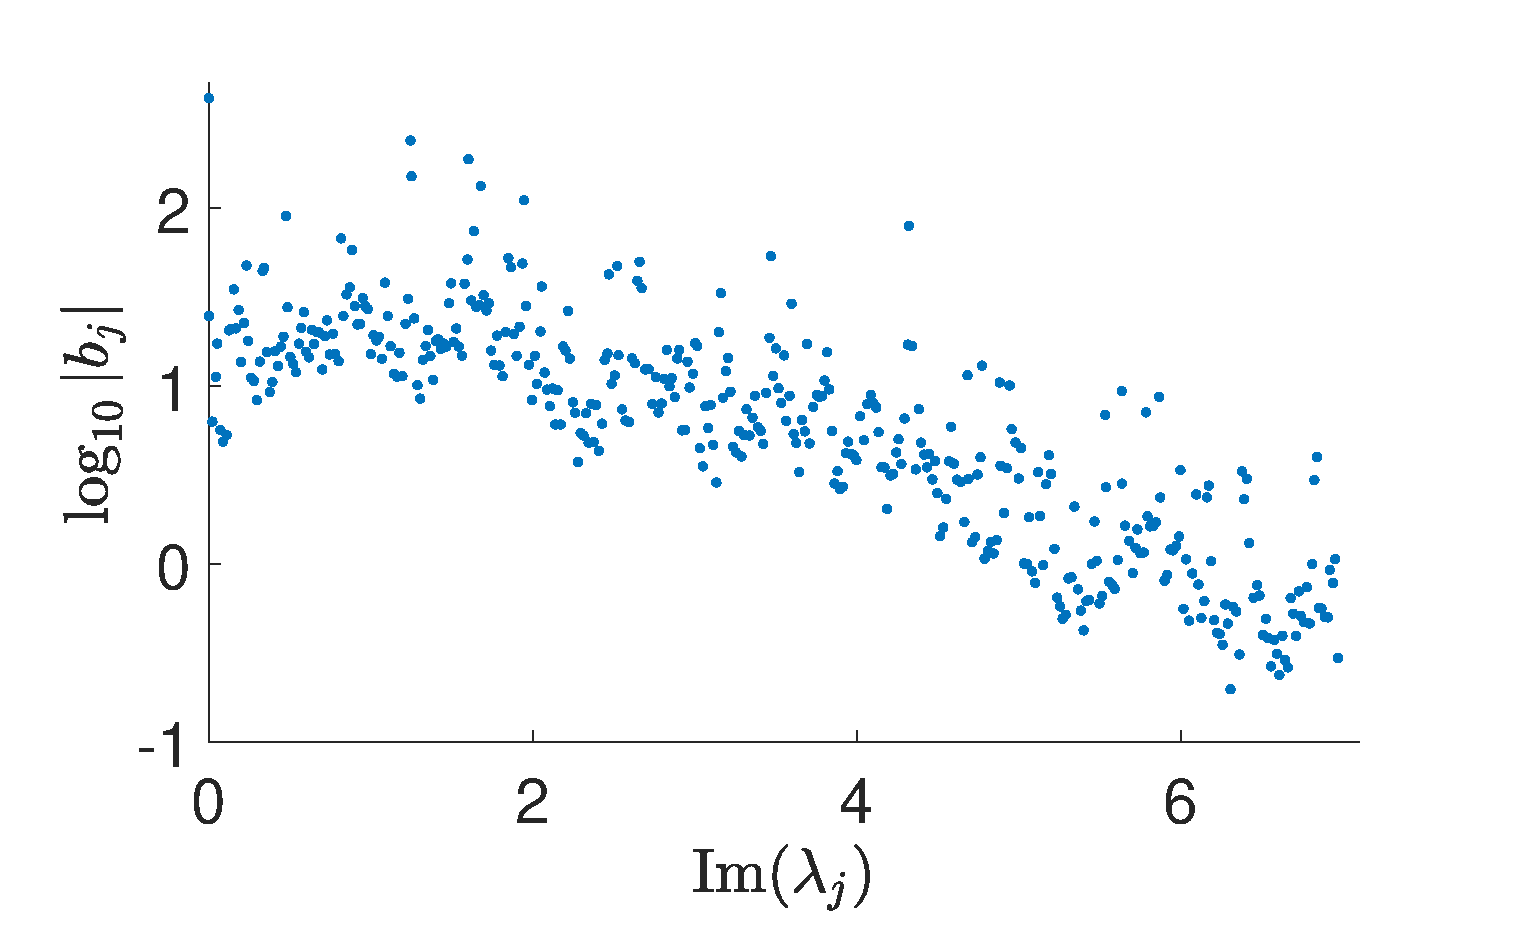
\includegraphics[width=.525\textwidth]{bvals_vs_imag_lam_hfforce_K_256_Lx_128_tf_2e4}\\
(e) HFS & (f) HFS
\end{tabular}
\caption{Plot of the real part of $\lambda_{j}$ against $\log_{10}|b_{j}|$ for the WWT (a), low-frequency saturated (c), and high-frequency saturated (e) regimes and the plot of the imaginary part of $\lambda_{j}$ against $\log_{10}|b_{j}|$  for the WWT (b), low-frequency saturated (d), and high-frequnecy saturated (f) regimes.}
\label{fig:wkosccomp}
\end{figure}
As seen in  Figures \ref{fig:wkosccomp} (a), (c), and (e) among those modes which are weakly-transitory, the mean always begins as the dominant mode with respect to its magnitude of $|b_{j}|$.  Likewise, we see from Figures \ref{fig:wkosccomp} (b), (d), and (f) that the higher temporal frequencies of oscillation correspond to smaller magnitudes of $|b_{j}|$, reflecting a kind of energy decay in time akin to what one usually sees via Fourier transforms in time or space.  However, focusing on the regime of weakly-transitory modes, we see marked differences in the spread of the magnitudes of $|b_{j}|$ with respect to the real part of the eigenvalues $\lambda_{j}$.  Thus, the way in which weakly transitory effects manifest themselves are distinguished in the different classes of flows.  

The impact of this manifests itself in the different dynamics and long time behavior of the compression ratio $C_{r}(n)$  seen in Figures \ref{fig:comprats} (a), (c), and (e) and the Jaccard indices $\mathcal{J}_{i}(n)$ seen in Figures \ref{fig:comprats} (b), (d), and (f).  As seen, the greater complexity of the WWT flow necessitates larger, and at times, more erratic numbers of modes in order to maintain the 90 \% threshold used for modal selection.  This likewise manifests as significant fluctuations in $\mathcal{J}_{i}(n)$ before it ultimately settles into a state in which the selected modes overlap by about 95 \%.   We also see the greater complexity of the HFS case in comparison to the LFS case by way of the overall larger compression ratio needed in the HFS case throughout most of the simulation.  Moreoever, we see that the Jaccard index is farm more volatile in the HFS case, with strong deviations in the choice of finite-dimensional subspace even up to close to the end of the simulation.  A partial explanation for this is that in the HFS case in order for energy to transfer to the longer wavelengths one must first form the higher frequency, spindle like structures seen in Figures \ref{fig:ampcomphf} (c)-(f).  Lastly, we note the presence of jumps in the compression ratio which clearly correspond to the more transitory modes, determined from examing the most leftward eigenvalues in Figures \ref{fig:comprats} (a), (c), and (e).

\begin{figure}[!ht]
\centering
\begin{tabular}{cc}
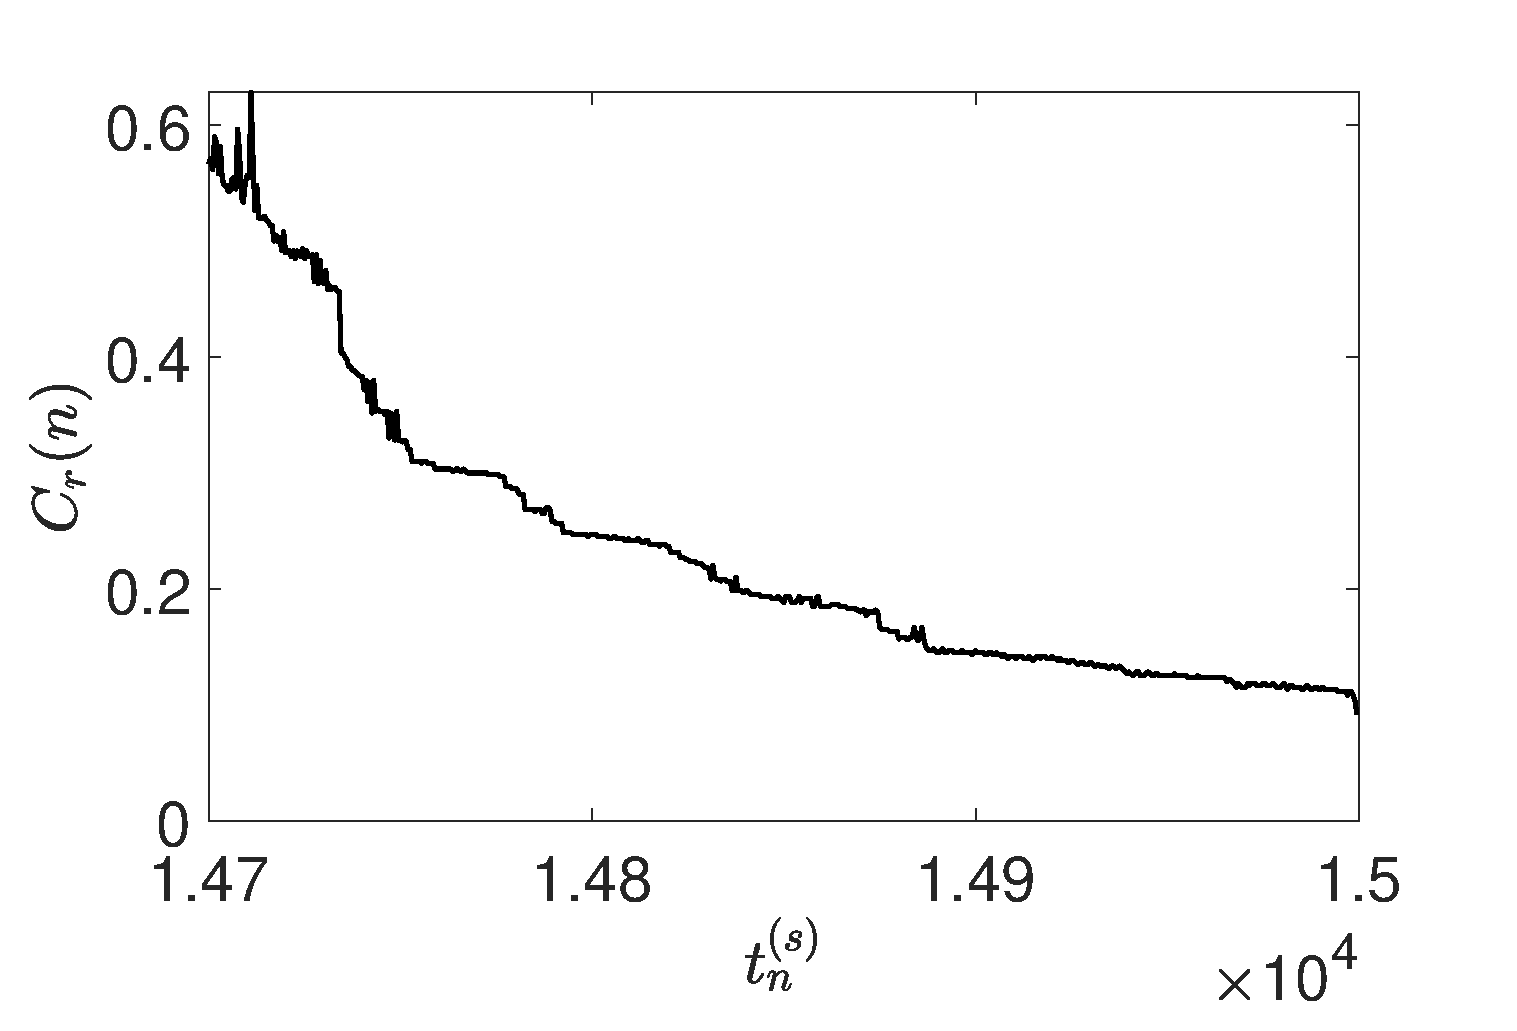
\includegraphics[width=.525\textwidth]{cratio_wwt_K_256_Lx_128_tf_1pt5e4} &\hspace{-25pt} 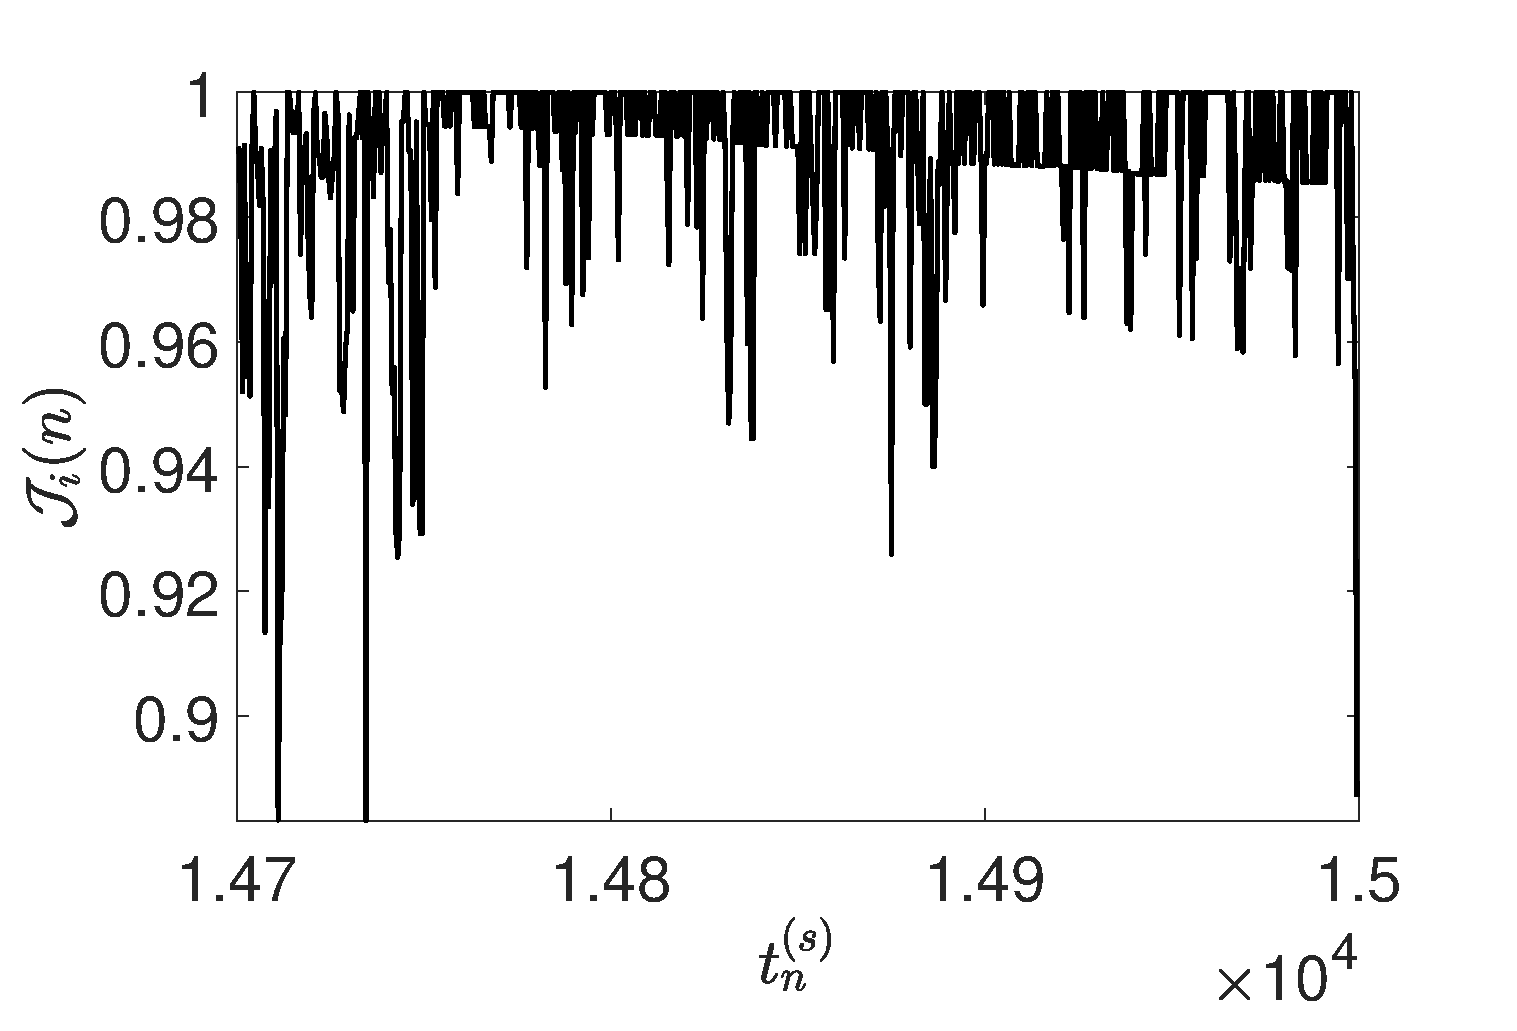
\includegraphics[width=.525\textwidth]{oratio_wwt_K_256_Lx_128_tf_1pt5e4}\\
(a) WWT & (b) WWT\\
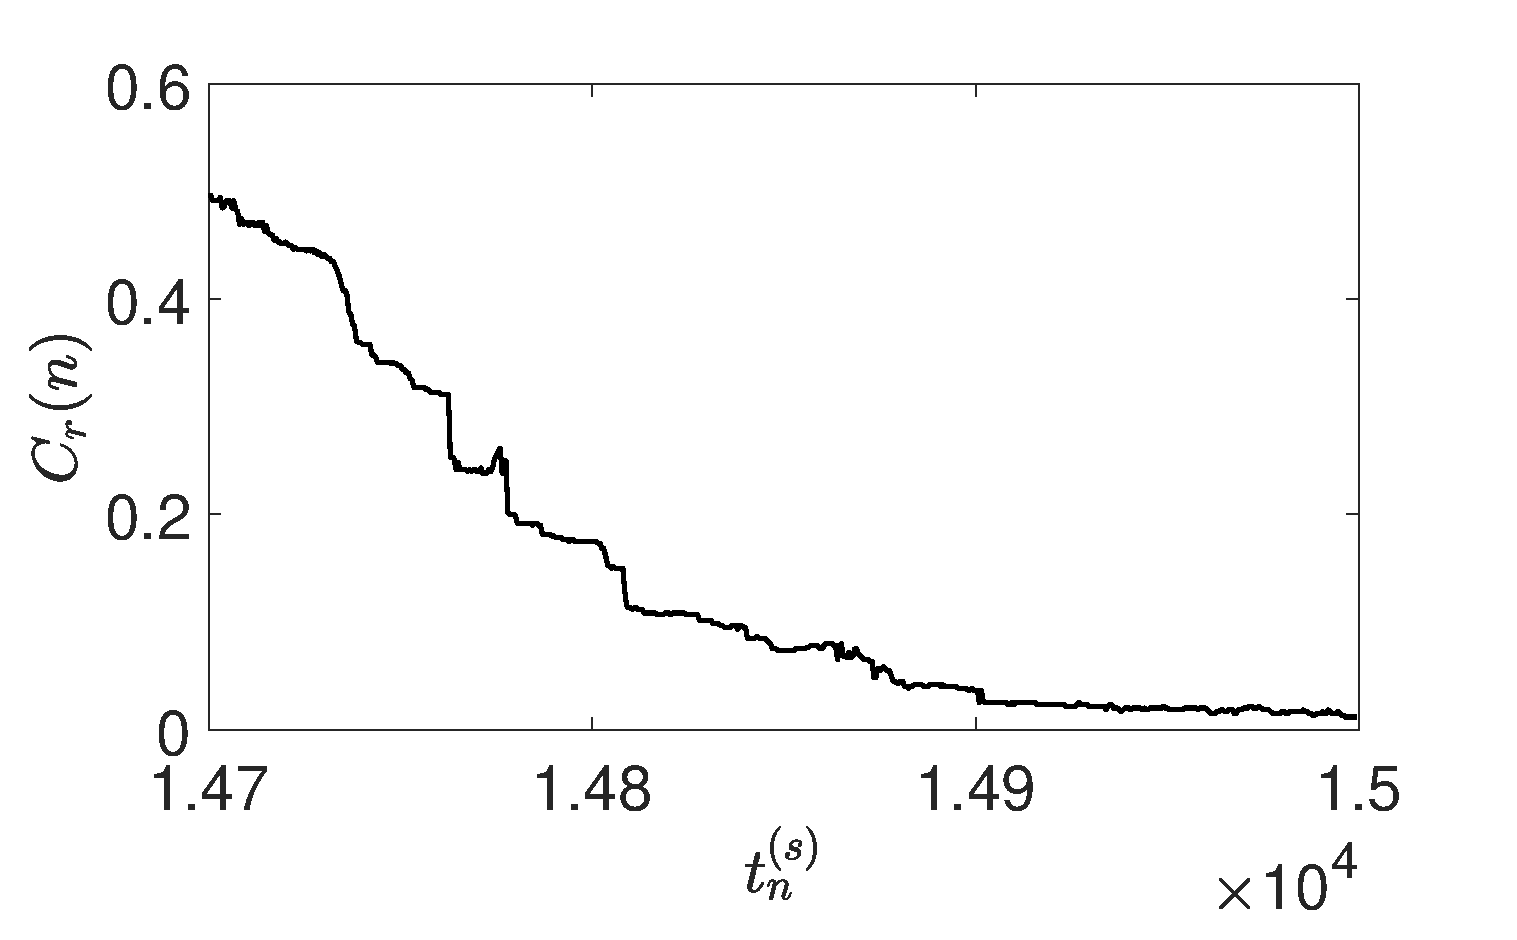
\includegraphics[width=.525\textwidth]{cratio_lfforce_K_256_Lx_128_tf_1pt5e4} &\hspace{-25pt} 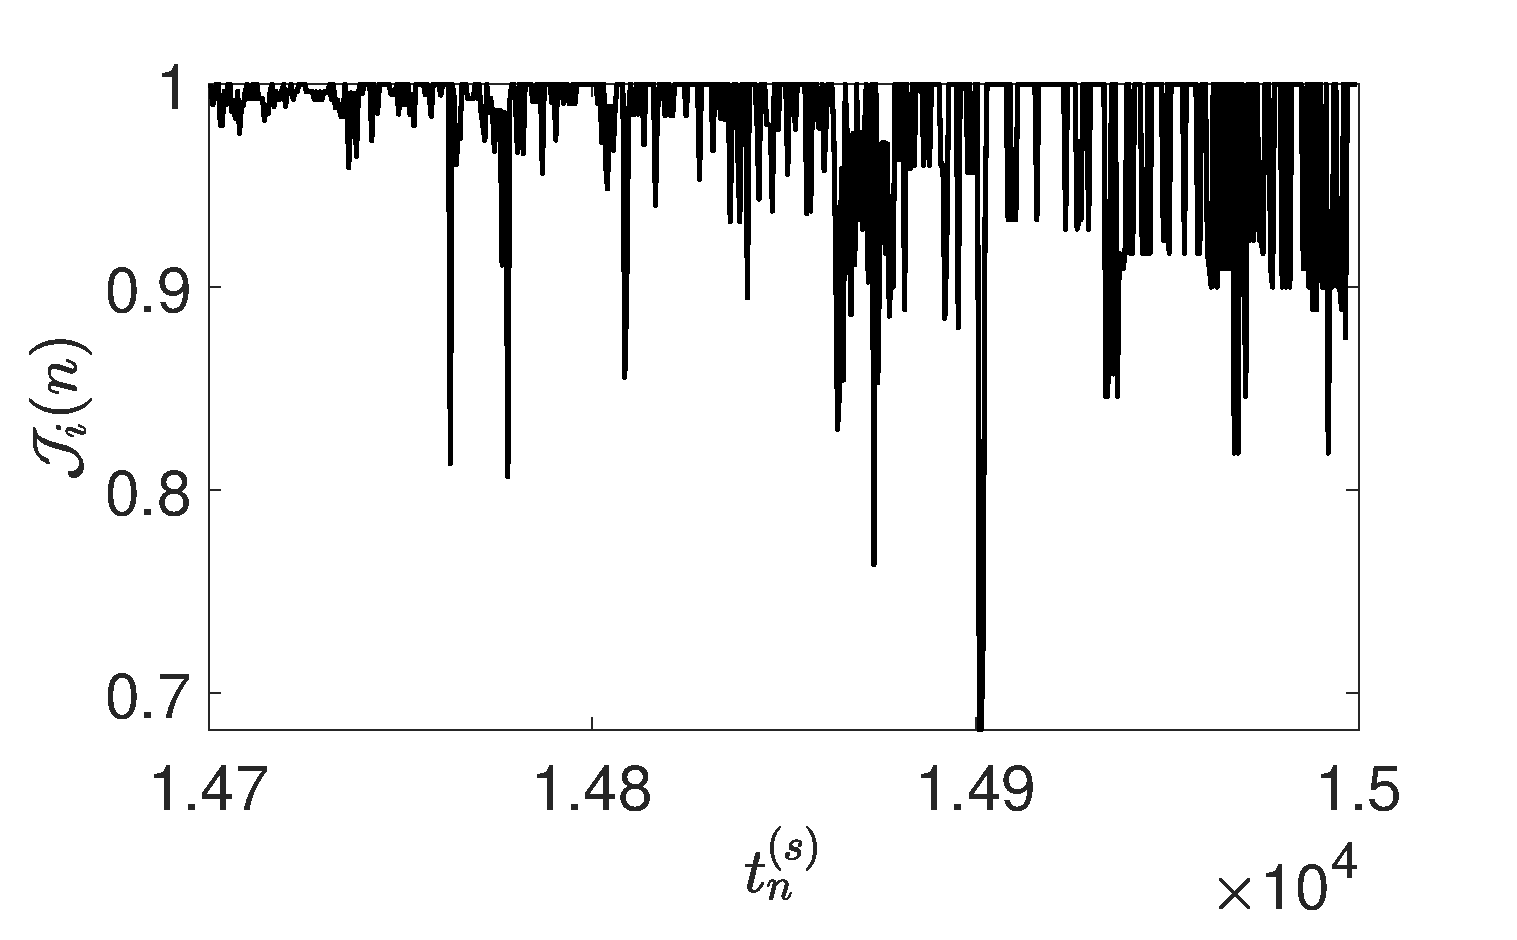
\includegraphics[width=.525\textwidth]{oratio_lfforce_K_256_Lx_128_tf_1pt5e4}\\
(c) LFS & (d) LFS\\
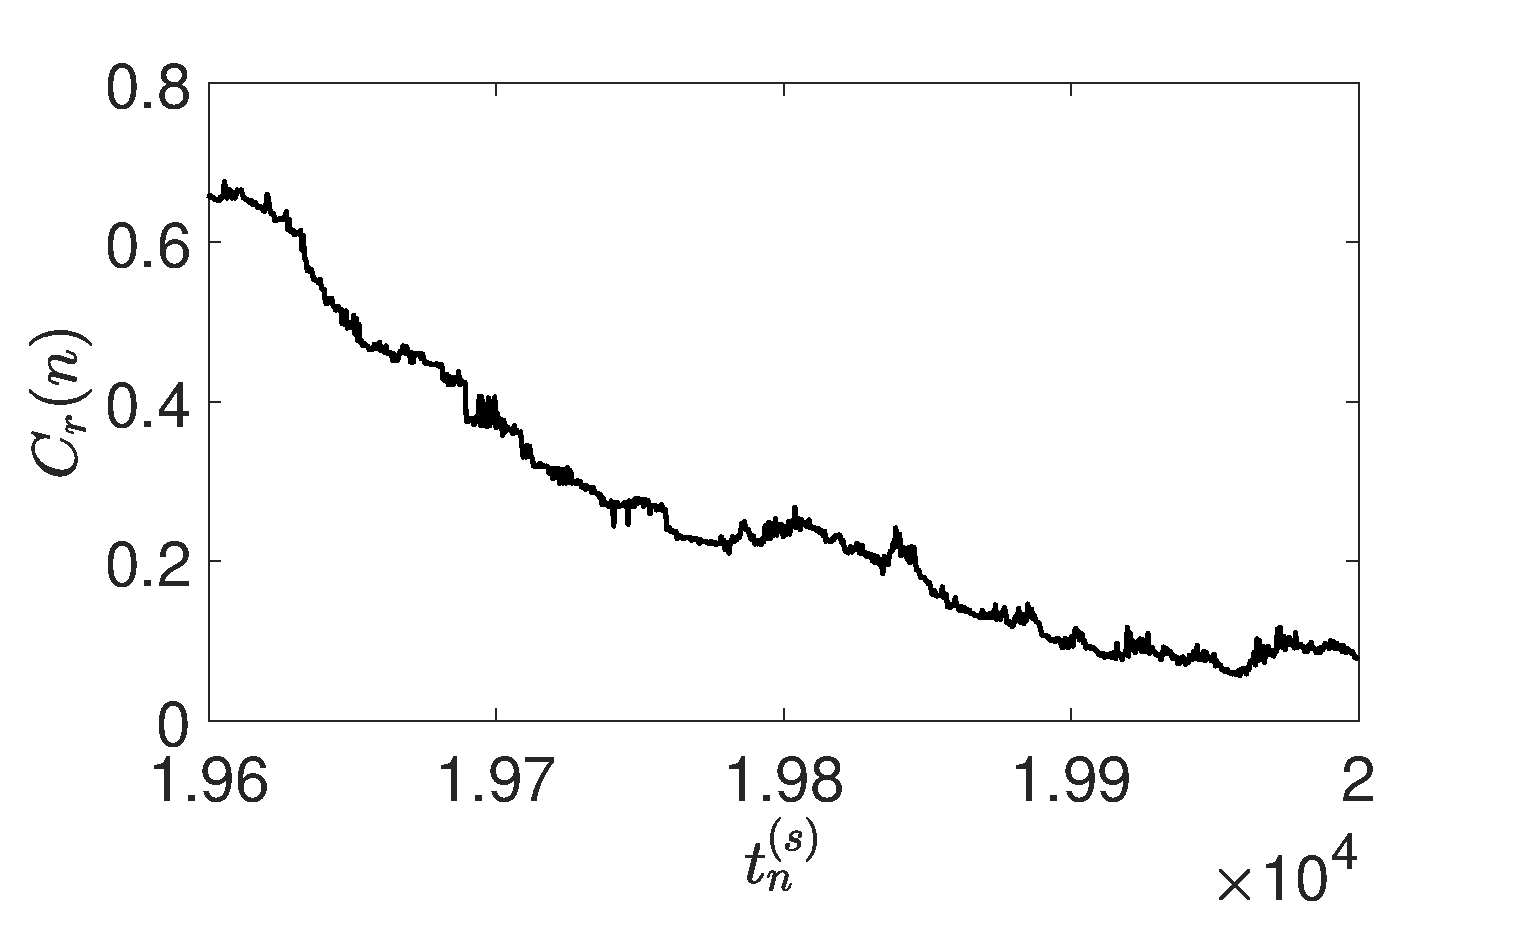
\includegraphics[width=.525\textwidth]{cratio_hfforce_K_256_Lx_128_tf_2e4} &\hspace{-25pt} 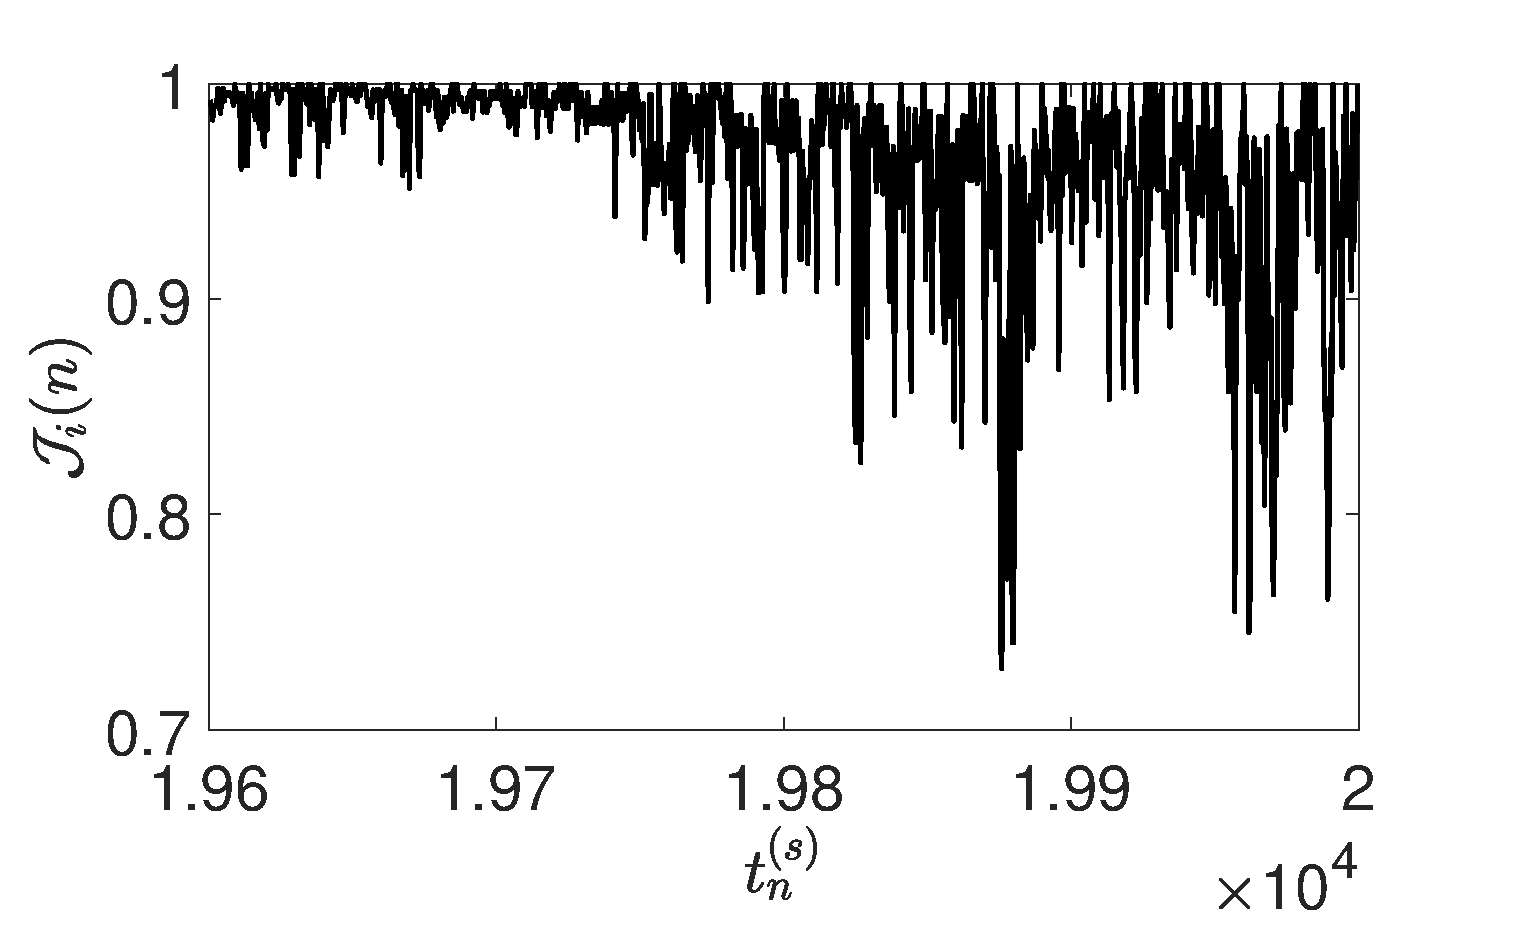
\includegraphics[width=.525\textwidth]{oratio_hfforce_K_256_Lx_128_tf_2e4}\\
(e) HFS & (f) HFS
\end{tabular}
\caption{Plot of the full spectrum for the WWT (a), low-frequency saturated (c), and high-frequency saturated (e) regimes and the compression ratio $C_{r}(n)$ for the WWT (b), low-frequency saturated (d), and high-frequnecy saturated (f) regimes.}
\label{fig:comprats}
\end{figure}

\section*{Conclusion}

\section*{Appendix}
\subsection*{Derivations Regarding Healing Lengths}
With units, our model of a BEC is given by the following Gross--Pitaevksii equation (GPE)
\[
i\hbar\psi_{t} = -\frac{\hbar^{2}}{2m}\Delta \psi + g\left| \psi\right|^{2}\psi, ~ g = \frac{4\pi \hbar^{2}a_{s}}{m}
\]
where $a_{s}$ is the `scattering length', and with the clear understanding that $\left|\psi\right|^{2}dxdy$ describes probabilities in the sense that 
\[
\int |\psi|^{2}dxdy = N,
\]
where we take $N$ to be the total number of particles under consideration.  Introducing the non-dimensionalizations 
\[
\tilde{x} = x/\lambda, ~ \tilde{y} = y/\lambda, ~ \tilde{t} = t/T, 
\]
and choosing
\[
\lambda^{2} = \frac{1}{8\pi |a_{s}|}, ~ T = \frac{m}{4\pi\hbar |a_{s}|}, 
\] 
then gives us
\[
i\psi_{t} = -\Delta \psi + \sigma\left| \psi\right|^{2}\psi,  ~\sigma = \mbox{sgn}(a_{s}).
\]

\bibliography{wwt}
\bibliographystyle{unsrt}

\end{document}